%%%%%%%%%%%%%%%%%%%%%%%%%%%%%%%%%%%%%%%%%%%%%%%%%%%%%%%%
%%% Plantilla desarrollada por Jorge Carrillo de Albornoz
%%% para los trabajos de Fin de Master del M�ster en
%%% Lenguajes y Sistemas Inform�ticos de la UNED
%%% Cualquier duda o comentario: jcalbornoz@lsi.uned.es
%%%%%%%%%%%%%%%%%%%%%%%%%%%%%%%%%%%%%%%%%%%%%%%%%%%%%%%%

\documentclass[a4paper,11pt,twoside,openright,spanish]{book}

\usepackage{latexsym}
\usepackage[latin1]{inputenc}
\usepackage[activeacute,spanish]{babel}
\frenchspacing
\usepackage{eucal}
\usepackage{multirow}
\usepackage{fancyhdr}
\usepackage[final,pdftex]{graphicx}
\usepackage{subfigure}
\usepackage{amsmath}
\usepackage{fullname_esp}
\usepackage[colorlinks=true, linkcolor=blue]{hyperref}
\usepackage{pdfpages}
\usepackage{algorithmic}
\usepackage{algorithm}
\usepackage{listings}
\lstset{
	basicstyle=\ttfamily,
	frame=single
}
\usepackage{color}
\usepackage{setspace}
\usepackage{caption}
\usepackage{booktabs}




%%%%%%%%%%%%%%%%%%%%%%%%%%%%%%%%%%%%%%%%%%%%%%%%%%%%%%%%
%%% SCRIPT DE TODO'S O TAREAS PENDIENTES CON BOCADILLOS.
%%%%%%%%%%%%%%%%%%%%%%%%%%%%%%%%%%%%%%%%%%%%%%%%%%%%%%%%
\usepackage{tikz}
\makeatletter \newcommand \listoftodos{\section*{Todo list} \@starttoc{tdo}}
\newcommand\l@todo[2]
    {\par\noindent \textit{#2}, \parbox{10cm}{#1}\par} \makeatother

\definecolor{orange}{rgb}{1,0.5,0}
\tikzstyle{notestyle} += [text width=\marginparwidth]
\tikzstyle{notestyleleft} += [text width=0.9\marginparwidth]
\tikzstyle{notestyle} = [draw=black, fill=orange, text width = 3cm]
\tikzstyle{notestyleleft} = [notestyle]
\tikzstyle{connectstyle} = [draw = orange, thick]
% Command for inserting a todo item
\newcommand{\todo}[1]{%
% Add to todo list
\addcontentsline{tdo}{todo}{\protect{#1}}%
%
\begin{tikzpicture}[remember picture, baseline=-0.75ex]%
    \node [coordinate] (inText) {};
\end{tikzpicture}%
%
% Make the margin par
\marginpar[%
{% Draw note in left margin
    \tikz[remember picture] \draw node[notestyleleft] (inNote) {#1};%
    \begin{tikzpicture}[remember picture, overlay]%
        \draw[connectstyle]
            ([yshift=-0.2cm] inText)
                -| ([xshift=0.2cm] inNote.east)
                -| (inNote.east);
    \end{tikzpicture}%
}%
]{% Draw note in right margin
    \tikz[remember picture] \draw node[notestyle] (inNote) {#1};%
    \begin{tikzpicture}[remember picture, overlay]%
        \draw[connectstyle]
            ([yshift=-0.2cm] inText)
                -| ([xshift=-0.2cm] inNote.west)
                -| (inNote.west);
    \end{tikzpicture}%
}%
}%

%%%%%%%%%%%%%%%%%%%%%%%%%%%%%%%%%%
%%%%%%%%%%%%%%%%%%%%%%%%%%%%%%%%%%

\floatname{algorithm}{Algoritmo}
\pagestyle{fancy}
\renewcommand{\chaptermark}[1]{\markboth{\textsc{Cap�tulo} \thechapter. #1}{}}
\renewcommand{\sectionmark}[1]{\markright{\thesection\ #1}}

\fancyhf{}
\fancyhead[LE,RO]{\thepage}
\fancyhead[LO]{\rightmark}
\fancyhead[RE]{\leftmark}

%% Dejar espacio para la regla
\renewcommand{\headrulewidth}{0.02cm} %Son 0.5pt

% Redefinici�n de 'plain' para la primera p�gina del cap�tulo
\fancypagestyle{plain}{
\fancyhf{}
\renewcommand{\headrulewidth}{0pt}
\renewcommand{\footrulewidth}{0pt}
}

% Limpiar las cabeceras de las p�ginas que quedan completamente blancas
\makeatletter
  \def\cleardoublepage{\clearpage\if@twoside \ifodd\c@page\else
  \vspace*{\fill}
    \thispagestyle{empty}
    \newpage
    \if@twocolumn\hbox{}\newpage\fi\fi\fi}
\makeatother


\setlength\headheight{20pt}


%%%%%%%%%%%%%%%%%%%%%%%%%%%%%%%%%%%%%%%%%%%%%%
%%% COMIENZA EL DOCUMENTO
%%%%%%%%%%%%%%%%%%%%%%%%%%%%%%%%%%%%%%%%%%%%%%

\pagenumbering{roman}
\makeindex
\begin{document}

\newlength{\centeroffset}
\setlength{\centeroffset}{-0.5\oddsidemargin}
\addtolength{\centeroffset}{0.5\evensidemargin}
\thispagestyle{empty}
\vspace*{\stretch{1}}
\setstretch{1.2}

\noindent
\hspace*{\centeroffset}

\renewcommand\contentsname{�ndice general}
\renewcommand\listfigurename{�ndice de Figuras}
\renewcommand\listtablename{�ndice de Tablas}
\renewcommand\bibname{Referencias}
\renewcommand\figurename{Figura}
\renewcommand\tablename{Tabla} 
\renewcommand\chaptername{Cap�tulo}
\renewcommand\appendixname{Ap�ndice}
\renewcommand\abstractname{Resumen}



%%%%%%%%%%%%%%%%%%%%%%%%%%%%%%%%%%%%%%%%%%%%%%
%%% PORTADA
%%%%%%%%%%%%%%%%%%%%%%%%%%%%%%%%%%%%%%%%%%%%%%

\thispagestyle{empty}
\vspace*{1cm}
\hrule
\mbox{ }

\begin{center}
\begin{LARGE}
Trabajo Fin de M�ster: Desarrollo de un sistema para la detecci�n del machismo en redes sociales \\ [0.3em]
\end{LARGE}
\end{center}

\hrule
\vspace*{1cm}
\begin{center}
 
\includegraphics[width=0.3\textwidth]{imagenes/Logo_UNED.jpg} %[width=4cm,,keepaspectratio]
\end{center}

\vfill
\begin{center}
  {\Large {\bf Trabajo Fin de M�ster}}
\end{center}

\vfill
\begin{center}
  \textbf{Francisco Miguel Rodr�guez S�nchez} \\ [0.2em]
  Trabajo de investigaci�n para el \\ \vspace{10pt}
  M�ster en Lenguajes y Sistemas Inform�ticos\\ \vspace{10pt}
  Universidad Nacional de Educaci�n a Distancia\\ \vspace{10pt}
  \vspace{2cm}
  Dirigido por \\ \vspace{10pt}
  \textbf{Dr. Jorge Amando Carrillo de Albornoz} \\ [0.5em]
  \textbf{Dr. Laura Plaza Morales} \\ [0.5em]
  Junio 2019\\
\end{center}


%%%%%%%%%%%%%%%%%%%%%%%%%%%%%%%%%%%%%%%%%%%%%%
%%% AGRADECIMIENTOS
%%%%%%%%%%%%%%%%%%%%%%%%%%%%%%%%%%%%%%%%%%%%%%
\chapter*{Agradecimientos}
\label{sec:Agradecimientos}

\noindent Agradecimientos si procede.


%%%%%%%%%%%%%%%%%%%%%%%%%%%%%%%%%%%%%%%%%%%%%%
%%% RESUMEN
%%%%%%%%%%%%%%%%%%%%%%%%%%%%%%%%%%%%%%%%%%%%%%
\chapter*{Resumen}
\label{sec:Resumen}
\noindent En el presente trabajo se propone una arquitectura para la detecci�n del machismo en la red de microblogging Twitter. El objetivo es comprender los mecanismos y se�ales textuales que conlleven actitudes o lenguaje machista en castellano. Para ello, se compone un corpus que contiene texto con contenido y expresiones machistas utilizando como fuente de datos la red social Twitter. Para la creaci�n del corpus, se desarrollar� una herramienta que recopilar� los mensajes creados en Twitter que contengan distintos t�rminos que pueden conllevar comportamientos machistas. Las expresiones o t�rminos que se buscan son aquellas que, de un modo u otro, minusvaloran el papel de las mujeres en nuestra sociedad, incentiven el abuso o acoso hacia las mujeres, o no les permita expresarse libremente. Existen gran cantidad de expresiones y t�rminos que se utilizan a diario de modo consciente o no que minimizan el papel de la mujer en la sociedad. Expresiones como ``feminazi'', ``ni�ata'' o ``a fregar'' han sido utilizadas para recopilar los tweets. Asimismo, utilizando el corpus generado, se desarrolla un sistema de clasificaci�n que permite detectar lenguaje machista de un modo automatizado. Se emplean distintos algoritmo de clasificaci�n y se establecen dos l�neas base que sirven como punto de partida para la evaluaci�n del sistema.

Finalmente, se ha realizado una evaluaci�n exhaustiva del sistema de clasificaci�n sobre el corpus creado para determinar su rendimiento. Los resultados obtenidos muestran que el procedimiento empleado es capaz de detectar el machismo en el corpus utilizado con un buen acierto. Sin embargo, se han detectado distintas limitaciones y problemas debido a la aproximaci�n empleada.



%%%%%%%%%%%%%%%%%%%%%%%%%%%%%%%%%%%%%%%%%%%%%%
%%% ABSTRACT
%%%%%%%%%%%%%%%%%%%%%%%%%%%%%%%%%%%%%%%%%%%%%%
\chapter*{Abstract}
\label{sec:Abstract}
\noindent The present work defines a new architecture to detect sexism at Twitter. The main goal is to understand the mechanism and textual signals which imply sexist attitudes or language of this kind in spanish. We create a new corpus which contains text with sexist expressions using the social network Twitter as main datasource. To create the corpus, a specific tool is developed to collect all the messages created at Twitter containing certains terms. We search for expressions which underestimate the role of women in our society, encourage the harassment towards them or limit their freedom of speech. There are many expressions used in a daily basis that underestimate the role of women in society. Terms such as ``feminazi'', ``ni�ata'' or ``a fregar'' have been used to collect tweets in our corpus. We also develop a classification system which allows us to identify sexist language in an automatic way. The system employs several machine learning algorithms and establish two baselines used as reference points for the system's evaluation.

Finally, an extensive evaluation is perfomed on the corpus to determine the perform of our approach in the classification task. The results obtained show that this procedure is able to identify sexism properly in the corpus used. However, some limitations and problems have been detected due to the approach used.



%%%%%%%%%%%%%%%%%%%%%%%%%%%%%%%%%%%%%%%%%%%%%%
%%% INDICES
%%%%%%%%%%%%%%%%%%%%%%%%%%%%%%%%%%%%%%%%%%%%%%
\tableofcontents
\listoffigures
\listoftables


%%%%%%%%%%%%%%%%%%%%%%%%%%%%%%%%%%%%%%%%%%%%%%
%%% ENTRADAS A LOS FICHEROS CON LOS CAPITULOS
%%%%%%%%%%%%%%%%%%%%%%%%%%%%%%%%%%%%%%%%%%%%%%
%%%%%%%%%%%%%%%%%%%%%%%%%%%%%%%%%%%%%%%%%%%%%%
%%% INTRODUCCION
%%%%%%%%%%%%%%%%%%%%%%%%%%%%%%%%%%%%%%%%%%%%%%

\chapter{Introducci�n}
\fancyhead[RE]{\textsc{CAP�TULO} \thechapter. Introducci�n}
\label{ch:Introduccion}
\pagenumbering{arabic}

\noindent El presente cap�tulo tiene como objetivo presentar al lector la motivaci�n y los objetivos del presente trabajo. Adem�s, se indica la estructura y los principales puntos abordados en el trabajo fin de m�ster. 

\section{Motivaci�n}
\label{sec:Motivacion}

\noindent Con el r�pido crecimiento de las redes sociales, la comunicaci�n entre personas de diferentes culturas en todo el mundo se produce de forma mucho m�s directa y sencilla. Esto provoca un gran aumento de ``ciber'' conflictos entre las personas que utilizan con frecuencia este tipo de plataformas. Con millones de contribuciones generadas diariamente por los usuarios de este tipo de herramientas, resulta impracticable y poco escalable implementar una pol�tica manual para detectar pr�cticas como el machismo o la xenofobia. Pese a esto, empresas como Facebook han anunciado planes para contratar varios miles de empleados encargados de moderar el contenido de la plataforma \cite{FacebookHiring2017}. Pese a dedicar muchos esfuerzos y recursos, las grandes compa��as como Twitter encuentran gran cantidad de dificultades para afrontar el problema \cite{Twitter2016} debido a la gran cantidad de posts que no pueden ser mediados por sus moderadores. Adem�s, han impulsado fuertes iniciativas para responder a las cr�ticas recibidas por no atajar el problema con la suficiente contundencia. Twitter, por ejemplo, ha aplicado pol�ticas para prohibir el uso de sus plataformas a quienes ataquen a personas o grupos sociales \cite{TwitterPolicy}. La importancia de este problema junto con la gran cantidad de informaci�n generada por los usuarios hace necesaria la creaci�n de sistemas y herramientas que puedan autom�ticamente detectar el contenido inapropiado en redes sociales.

Un nuevo estudio realizado en EEUU \cite{Duggan2017} sostiene que el 41\% de personas encuestadas hab�a sufrido personalmente alg�n tipo de discriminaci�n o acoso online, de las cuales el 18\% hab�a sufrido alg�n tipo de acoso grave, por ejemplo debido a su g�nero (8\%). De igual modo, las mujeres tienen m�s de el doble de probabilidades de sufrir acoso debido a su g�nero \cite{Duggan2017}.

El problema es a�n m�s grave si se tiene en cuenta que un abuso verbal en redes sociales puede acarrear un acto de violencia f�sica. No solo es importante por el propio mensaje, este tipo de plataformas permiten propagar un mensaje machista que incita al odio, al menosprecio o a la desigualdad. De hecho, no es inusual que contenidos machistas hacia las mujeres sean trasladados a acciones violentas. Por ejemplo, algunos estudios sociales como \cite{Fulper2014} demuestra la existencia de una correlaci�n entre el n�mero de violaciones y el n�mero de tweets machistas por estado en USA. Esto sugiere que las redes sociales pueden ser utilizadas como detector de violencia machista e incluso pueden ayudar a anticiparla o prevenirla.

Amnist�a internacional public� recientemente un estudio donde denuncia este hecho \cite{Amnesty2017}. En el reporte, se explica c�mo para muchas mujeres Twitter es una plataforma donde la violencia y al abuso contra ellas florece, en la mayor�a de los casos, sin ninguna consecuencia. Seg�n este informe, Twitter est� fallando como empresa a la hora de respetar los derechos de la mujer en l�nea. En lugar de reforzar las voces de las mujeres, la violencia y el abuso que experimentan en la plataforma hace que las mujeres se autocensuren a la hora de postear, limiten sus interacciones e incluso les hace abandonar Twitter por completo. De este modo, la violencia y el abuso que muchas mujeres experimentan en Twitter tiene un efecto perjudicial en su derecho a expresarse en igualdad, libremente y sin miedo. 

Todos los estudios listados justifican la necesidad de detectar y filtrar de un modo automatizado el contenido que incita o promueve el machismo. En concreto, el lenguaje machista o sexista, ocupa gran parte de este discurso en sitios webs como Twitter. Mientras que en la mayor�a de las plataformas el uso de este tipo de lenguaje est� prohibido, el tama�o de estas redes hace imposible controlar todo el contenido que generan. Resulta adecuado, por tanto, afirmar que las posibilidades y ventajas que proporcionar�a un sistema capaz de detectar este tipo de actitudes en en texto de manera autom�tica supondr�an un beneficio sustancial para los usuarios y consumidores de redes sociales e internet en general. Todo lo expuesto justifica, sin duda, la realizaci�n de este trabajo en el que se propone una arquitectura para la detecci�n autom�tica del machismo. 


\section{Propuesta y objetivos}
\label{sec:PropuestaYObjetivos}

\noindent El trabajo realizado en este proyecto presenta un sistema de clasificaci�n autom�tico para la detecci�n del machismo en redes sociales. El abuso online se ha convertido en un gran problema, especialmente por el anonimato y la interactividad de la web que facilita el incremento y permanencia de este tipo de abusos. Se trata de un campo en el que ha aumentado la producci�n cient�fica enormemente durante este mismo a�o y donde se han desarrollado competiciones con gran participaci�n por parte de la comunidad cient�fica \cite{AMIOverview2018}.

Los atributos utilizados para la tarea de clasificaci�n  se agrupan en 3 tipos: variables categ�ricas, num�ricas y texto. Para cada atributo, se aplican diferentes m�todos como la tokenizaci�n, el escalado o la sustituci�n de emoticonos. Tras esto, se unifican los distintos tipos de atributos procesados en un conjunto de datos com�n que ser� la entrada de la �ltima fase. En la �ltima etapa, se emplean algoritmos de clasificaci�n supervisada con la intenci�n de obtener un modelo predictivo capaz de detectar las se�ales textuales que expresan lenguaje machista. A lo largo del trabajo, se presenta el ciclo completo para la recolecci�n de datos, preprocesamiento y construcci�n del sistema de clasificaci�n para el lenguaje.

Para el correcto funcionamiento de estos sistemas de clasificaci�n supervisados se necesitan ejemplos previamente etiquetados con los que entrenar el algoritmo. En este caso, se ha desarrollado un corpus mediante la b�squeda de 29 t�rminos o expresiones utilizando como fuente de datos la red social Twitter. Este corpus est� compuesto por 3600 mensajes y ha sido etiquetado en 3 categor�as: MACHISTA, NO\_MACHISTA Y DUDOSO. De este modo, este trabajo realiza una aportaci�n importante mediante este corpus etiquetado compuesto por un gran n�mero de expresiones y actitudes machistas.


\section{Estructura del documento}
\label{sec:EstructuraDelDocumento}

\noindent En este cap�tulo se estructuran los cap�tulos que componen el presente trabajo fin de m�ster.

\begin{description}

\item \textbf{Cap�tulo 1. Introducci�n.} Este cap�tulo introduce los principales motivos que han llevado a la realizaci�n de este trabajo, as� como la problem�tica y el estado actual de la disciplina. Por �ltimo, se presentan las diferentes contribuciones del trabajo realizado.
\item \textbf{Cap�tulo 2. Estado del arte.} Este cap�tulo describe en mayor detalle la disciplina que nos ocupa, presentando su origen y su historia hasta el presente. Se muestran las t�cnicas actuales m�s utilizadas para resolver las tareas m�s relevantes del tema abordado, as� como sus debilidades.
\item \textbf{Cap�tulo 3. Herramientas utilizadas.}  En este cap�tulo se describen todas las herramientas y tecnolog�as que han sido necesarias para elaborar el proyecto. Se realiza una definici�n de cada una de ellas y se describe el papel que desempe�an dentro del trabajo desarrollado.
\item \textbf{Cap�tulo 4. MeTwo dataset (Machismo and Sexism Twitter Identification dataset)}  En este cap�tulo se describe en profundidad la metodolog�a seguida para componer el corpus con texto y expresiones machistas.
\item \textbf{Cap�tulo 5. Sistema.}  En este cap�tulo se describe en profundidad el sistema de clasificaci�n propuesto.
\item \textbf{Cap�tulo 6. Evaluaci�n y discusi�n.} Este cap�tulo describe la metodolog�a utilizada para evaluar la propuesta realizada, a la vez que presenta los resultados obtenidos al evaluar el m�todo propuesto en diferentes tareas y sobre colecciones de evaluaci�n de distintos dominios. Adem�s, se analiza y discute en profundidad los resultados obtenidos en la evaluaci�n presentada anteriormente.
\item \textbf{Cap�tulo 7. Conclusiones y trabajo futuro.} Este cap�tulo recopila las diferentes conclusiones extra�das del trabajo realizado, y propone algunas l�neas de trabajo futuro.

\end{description}
%%%%%%%%%%%%%%%%%%%%%%%%%%%%%%%%%%%%%%%%%%%%%%%%%%%
%%% ESTADO DEL ARTE
%%%%%%%%%%%%%%%%%%%%%%%%%%%%%%%%%%%%%%%%%%%%%%%%%%%

\chapter{Estado del arte}
\fancyhead[RE]{\textsc{CAP\'ITULO} \thechapter. Estado del arte}
\label{ch:EstadoArte}

\noindent El presente cap�tulo tiene como objetivo presentar al lector la detecci�n del lenguaje machista en redes sociales. Para ello, se realizar� una revisi�n de los trabajos m�s relevantes en la tarea de detecci�n de lenguaje abusivo y machista, en los que se analizar�n los or�genes de esta tarea, las soluciones t�cnicas y las aportaciones m�s relevantes.


\section{Clasificaci�n de textos}
\label{sec:Ejemplo_seccion}

\noindent El procesamiento del lenguaje natural (\textit{``Natural Language Processing''}, NLP) tiene como objetivo fundamental el desarrollo de m�todos que permitan a los computadores realizar tareas relacionadas con el lenguaje humano, como la comunicaci�n o el procesamiento de textos. La principal diferencia del NLP con el resto de l�neas de investigaci�n relacionadas con el an�lisis de datos o la inteligencia artificial es la necesidad de un conocimiento del lenguaje en todas sus aplicaciones. Elementos clave del lenguaje como la fon�tica, la fonolog�a, la morfolog�a, la sintaxis, la sem�ntica, la pragm�tica y la discursiva son esenciales en cualquier t�cnica de procesamiento del lenguaje \cite[Cap�tulo~1]{Jurafsky}.

Una de las �reas m�s importantes de investigaci�n relacionadas con el NLP es la clasificaci�n de textos o documentos. De un modo general, se conoce como clasificaci�n autom�tica \cite[Cap�tulo~4]{Jurafsky} a la tarea de asignar una o varias categor�as predefinidas sobre una colecci�n de instancias a clasificar. Del mismo modo, la clasificaci�n de textos \cite[Cap�tulo~4]{Jurafsky} se puede entender como aquella tarea en la que un documento o texto es etiquetado como perteneciente a un determinado conjunto. Este tipo de t�cnicas se utilizan para un gran n�mero de aplicaciones, tales como:
\begin{itemize}
	\itemsep0em 
	\item Indexaci�n para sistemas de recuperaci�n de informaci�n \cite[Chapter~17]{Jurafsky}
	\item Detecci�n de \textit{spam} \cite{Hai2010,Jurafsky}
	\item Identificaci�n del lenguaje \cite[Chapter~3]{Jurafsky}
	\item An�lisis de sentimientos \cite[Chapter~4]{Jurafsky}
	\item Organizaci�n de documentos \cite{Mauro2016}
	\item Desambig�aci�n del sentido de las palabras \cite{Russell2002}
	\item Filtrado de textos \cite{Mark}
\end{itemize}

Formalmente, el problema se define como un texto o documento $d$ que puede pertenecer a un conjunto fijo de clases $C=\{c_1,c_2,...,c_i\}$. La salida del sistema es la predicci�n la clase $c \in C$.

Para resolver el problema de la clasificaci�n de textos existen dos enfoques principales: uno basado en reglas y otro mediante algoritmos de clasificaci�n supervisado.

Los sistemas basados en reglas utilizan patrones predefinidos por un experto para crear un conjunto de pautas mediante la combinaci�n de palabras u otros atributos \cite{Elizabeth2001}. En este tipo de arquitecturas, la precisi�n puede ser alta siempre que estas reglas est�n cuidadosamente seleccionadas por un experto. Sin embargo, dichos sistemas resultan muy costosos de construir y mantener. Adem�s, se trata de sistemas muy espec�ficos para un dominio o problema concreto, y dif�cilmente trasladables a un dominio distinto.

El aprendizaje supervisado se construye sobre un conocimiento a priori. Se debe disponer de un conjunto de documentos de ejemplo para cada una de las categor�as consideradas. Despu�s de una etapa de entrenamiento, el sistema queda ajustado de modo que, ante nuevos ejemplos, el algoritmo es capaz de clasificarlos en alguna de las clases existentes. Para este tipo de sistemas se utilizan distintos modelos de clasificadores: \textit{Naive Bayes}, \textit{Regresi�n log�stica}, \textit{SVM}, \textit{redes neuronales}, etc \cite{Aurangzeb2010}.

Para construir cualquier clasificador de textos o documentos es necesario seguir los siguientes pasos:

\begin{itemize}
	\itemsep0em 
	\item Extraer los atributos o \textit{features} necesarias para realizar una representaci�n fiel del texto y que permita la utilizaci�n de un algoritmo de clasificaci�n
	\item Desarrollar procedimientos por los cuales los documentos puedan ser clasificados autom�ticamente dentro de
	categor�as.
	\item Evaluar la calidad de la clasificaci�n en relaci�n a alg�n criterio.
\end{itemize}


\subsection{Representaci�n textual}
\label{sec:Ejemplo_subSeccion} 


\subsubsection{Modelo de espacio vectorial}
\label{sec:Ejemplo_subSeccion} 

\noindent La representaci�n del texto es un paso fundamental para el procesamiento autom�tico de textos. Una representaci�n fiel al contenido del documento, que incluya la informaci�n necesaria para extraer conocimiento �til, ser� clave para el desarrollo de una arquitectura con un rendimiento adecuado. En este proceso, se han de tener en cuenta las especificaciones de los algoritmos que se empleen a continuaci�n.

En esta fase, se definen todos los atributos utilizados en el paso posterior por el algoritmo de clasificaci�n. Los atributos seleccionados o generados a partir de los originales ser�n los que marquen el �xito de la arquitectura completa. La elecci�n del algoritmo de clasificaci�n para los pasos posteriores influir� de un modo mucho menos significativo. Por ejemplo, en \cite{Victor2018} y \cite{Wahyu2018} se utiliza el mismo algoritmo de clasificaci�n pero los resultados son muy diferentes debido a los atributos utilizados. 

Un modelo de representaci�n muy utilizado se conoce como modelo de representaci�n vectorial \cite{Fresno2006}. Mediante esta representaci�n, los documentos se modelan como vectores dentro de un espacio eucl�deo. De este modo, se pueden aplicar operaciones de distancia entre vectores, como indicador de su cercan�a seg�n el contenido textual. En la siguiente imagen se muestra un ejemplo en dos dimensiones:

\begin{center}
	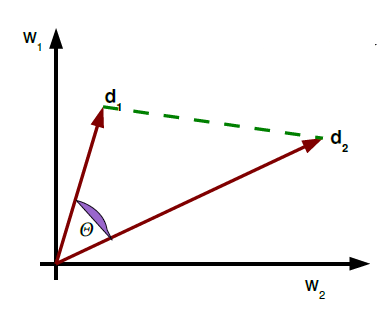
\includegraphics[width=0.4\textwidth]{imagenes/modelo_vectorial.png} %[width=4cm,,keepaspectratio]
	\captionof{figure}{Representaci�n vector de documentos}	
\end{center}

En este caso, se tendr�a un vocabulario con �nicamente dos rasgos $w_1$ y $w_2$ que conforman el espacio en el que se encuentran los documentos o textos $d_1$ y $d_2$. De este modo, se pueden emplear medidas de distancia, como la distancia eucl�dea o la distancia coseno, para comparar ambos documentos.

Utilizando este modelo, un texto quedar� representado como una combinaci�n lineal de vectores, donde cada coeficiente representa la relevancia de cada rasgo en el contenido del texto, calculado con una funci�n de pesado. Para un texto $d$, un vocabulario de tama�o $n$: $\vec{d}=t_1j \vec{t_1} + ... + t_nj \vec{t_n} $. Para el c�lculo de la relevancia de cada rasgo $t_nj$, se utilizar� una funci�n de pesado. Una de las m�s utilizadas se conoce como TF-IDF (frecuencia del termino x frecuencia inversa del documento) y se calcular�a del siguiente modo: \[TF-IDF(\vec{t_i},\vec{d_j})=f_{ij}\log(\frac{N}{d_f(\vec{t_i})})\] donde $N$ es la dimensi�n del corpus (en este caso n�mero de tweets), $f_{ij}$ la frecuencia del t�rmino en el documento y $d_f(\vec{t_i})$ el n�mero de documentos (en este caso el tweet) en los que aparece el t�rmino.


\subsubsection{Representaci�n sem�ntica mediante modelo de espacio vectorial}
\label{sec:Ejemplo_subSeccion} 

\noindent En el apartado anterior, se ha descrito un procedimiento para la representaci�n textual que permite expresar la informaci�n contenida en el texto como una combinaci�n lineal de vectores, donde cada coeficiente representa la existencia o no de los t�rminos contenidos en el vocabulario del corpus. Sin embargo, una desventaja de este m�todo es su incapacidad para representar la informaci�n sem�ntica de los documentos. Es decir, este m�todo no es capaz de capturar informaci�n acerca del significado o concepto que contienen los t�rminos presentes en los documentos. Por ejemplo, consid�rense los siguientes documentos:

	$d_1 = $``\textit{Pizza margarita}''

	$d_2 = $``\textit{Pizza calzone}''

	$d_3 = $``\textit{Macarrones}''

% Please add the following required packages to your document preamble:
% \usepackage{booktabs}
\begin{table}[]
	\centering
	\begin{tabular}{@{}lllll@{}}
		\toprule
		\textbf{T�rminos} & \textbf{Pizza} & \textbf{margarita} & \textbf{calzone} & \textbf{Macarrones} \\ \midrule
		\textbf{$d_1$} & 1 & 1 & 0 & 0 \\
		\textbf{$d_2$} & 1 & 0 & 1 & 0 \\
		\textbf{$d_3$} & 0 & 0 & 0 & 1 \\ \bottomrule
	\end{tabular}
	\caption{Matriz documento - t�rmino}
	\label{tab:my-table}
\end{table}

Si se realiza una representaci�n de los documentos seg�n el modelo descrito anteriormente (con el n�mero de t�rminos como funci�n de pesado) se obtendr�a la matriz de la tabla 2.1. Como se puede observar, los documentos $d_1$ y $d_2$ tienen en com�n un atributo mientras que el documento $d_3$ no tendr�a ning�n rasgo com�n con el resto de documentos. Sin embargo, si se tiene en cuenta el significado o el concepto que expresan los documentos, se concluir�a que todos los documentos representan comida italiana y, por tanto, todos tienen en com�n ese rasgo sem�ntico. Esto indica que si un documento se trata �nicamente como una sucesi�n de t�rminos, se perder�n los conceptos a los que hace referencia.

Los m�todos para la generaci�n autom�tica de atributos sem�nticos fueron desarrollados alrededor del a�o 1990 con el objetivo de capturar la informaci�n sem�ntica o los conceptos presentes en los documentos. Uno de los algoritmos m�s populares dentro de esta familia se conoce como LSA (\textit{Latent Semantic Analysis}) \cite{Deerwester1990} que describe a cada palabra o conjunto de palabras en un espacio vectorial de dimensi�n reducida en el que las palabras sem�nticamente similares se encontrar�n m�s pr�ximas. Para ello, este m�todo toma como entrada una matriz t�rmino-documento a la que se le aplica una descomposici�n de valores singulares (\textit{Singular Value Descomposition}, SVD) obteniendo as� una representaci�n vectorial tanto de los t�rminos como de los documentos. De este modo, se puede cuantificar la similitud sem�ntica de dos palabras mediante el uso de medidas de distancias entre vectores. Esta t�cnica fue r�pidamente aplicada a distintos dominios como la representaci�n de un modelo cognitivo \cite{Landauer1997}, modelo de lenguaje \cite{Jurafsky1998} o calificador autom�tico \cite{Rehder1998}.

Aunque el m�todo LSA se plante� como una variante al modelo de espacio vectorial, hace uso de las mismas formas de representaci�n a la entrada del m�todo. Aqu�, el texto se representa en un espacio de coordenadas donde los documentos y los t�rminos se expresan como una combinaci�n de factores sem�nticos o \textit{topics} subyacentes. De este modo, cuando las palabras est�n relacionadas, por ejemplo, ``\textit{Pizza}'', ``\textit{Lasa�a}'' y ``\textit{Macarrones}'', cabr� esperar que aparecieran en conjuntos similares de documentos. 

Formalmente, el LSA es la aplicaci�n de la funci�n SVD a la matriz t�rmino documento. Esta matriz $A_{[mxn]}$ almacena en sus componentes $a_{ij}$ informaci�n relativa a las frecuencias de los t�rminos $t_i$ en los documentos $d_j$. Un ejemplo de esta matriz se obtendr�a aplicando la transpuesta $A^T$ a la matriz traspuesta de la tabla 2.1. La proyecci�n SVD se calcula descomponiendo la matriz $A_{[mxn]}$ en un producto de tres matrices:


\[A_{[mxn]}=U_{[mxr]}\Sigma_{[rxr]}(V_{[nxr]})^T\] donde $r$ toma valores entre 1 y $\min(\dim(\vec{t_i}, d))$. Este valor $r$ se puede considerar como el n�mero de rasgos sem�nticos o \textit{topics} (temas) en los que se agrupar�n los documentos. En esta expresi�n, las matrices $V$ y $U$ est�n formadas por vectores ortonormales (el m�dulo de cada vector columna es 1 y todos ellos son linealmente independientes). De este modo, $V^T V = U^T U = I$ mientras que $\Sigma$ representa una matriz diagonal en la que sus elementos est�n ordenados en orden decreciente.

En resumen, SVD encuentra la proyecci�n �ptima a un espacio de dimensi�n reducida explotando patrones de coaparici�n entre t�rminos. En este proceso, aquellos rasgos que tienen patrones similares son proyectados a una misma direcci�n. Estos patrones tratan de inferir similitud sem�ntica entre t�rminos, lo que en ocasiones no es acertado \cite{Manning1990}. Sin embargo, en muchos casos ha demostrado ser un indicador v�lido de relaciones tem�ticas. En \cite{Foltz1996}, la representaci�n del documento se reduce a un conjunto de 20 palabras y se consideran conjuntos de sintagmas, tratados como atributos, para crear el vector de caracter�sticas, usando la similitud normalizada entre fragmentos de textos.


\subsubsection{\textit{Word Embedding}}
\label{sec:Ejemplo_subSeccion}

\noindent En las secciones previas se han presentado dos m�todos que hacen uso del modelo de espacio vectorial para representar los documentos. En el primer apartado, se explic� c�mo representar texto mediante un vector en el que las dimensiones corresponden a las palabras en el vocabulario. En esta secci�n, se presenta un m�todo alternativo para representar t�rminos mediante el uso de vectores de n�meros reales de menor tama�o y m�s densos (m�s valores distintos de cero). Este tipo de t�cnicas se conocen como \textit{word embedding} y han tenido un �xito enorme en numerosas tareas relacionadas con el procesamiento natural del lenguaje en los �ltimos a�os \cite{Jacob2019} superando a los m�todos empleados tradicionalmente como la t�cnica LSA \cite{Baroni2014} presentada en el apartado anterior. Mientras que los m�todos explicados hasta ahora utilizan el conteo de t�rminos para representar los documentos, los m�todos basados en \textit{word embedding} pueden ser vistos como modelos de predicci�n que intentan predecir los t�rminos alrededor de las palabras (o a la inversa). De este modo, estos m�todos son capaces de tener en cuenta el contexto en el que se utilizan los t�rminos presentes en el corpus, consiguiendo as� capturar la informaci�n sem�ntica en su representaci�n.

Como se ha comentado, los vectores obtenidos mediante \textit{word embedding} son m�s densos y funcionan mejor que las representaciones tradicionales. Aunque no se entienden todas las razones de esta mejora, se tienen ciertas ideas \cite[Cap�tulo~6]{Jurafsky}. Primero, estos vectores pueden utilizarse de un modo m�s adecuado como atributos en los sistemas de aprendizaje de m�quina debido a la gran reducci�n de los vectores con los que se trabaja. Asimismo, esta reducci�n de coeficiente puede ayudar a mejorar la capacidad de generalizaci�n del clasificador y prevenir el sobreajuste. Finalmente, las t�cnicas de \textit{word embedding} son capaces de capturar la informaci�n sem�ntica de los t�rminos. Por ejemplo, los documentos de la tabla 2.1 ser�n pr�ximos entre s� si se utilizaran este tipo de m�todos para representar los t�rminos que contienen.

El t�rmino \textit{word embeddings} fue originalmente acu�ado en \cite{Bengio2003}, sin embargo, fue en  \cite{Collobert2008} donde se demostr� todas las ventajas de este tipo de metodolog�a. Otro hito importante dentro de esta l�nea de trabajo fue la publicaci�n de \cite{Mikolov2013} en la que se presenta la librer�a \textit{word2vec}, una de las herramienta m�s populares que permite entrenar y utilizar modelos pre-entrenados de \textit{word embedding}. Un a�o despu�s, fue presentado \textit{GloVe} \cite{Pennington2014} confirmando la popularidad de las t�cnicas de \textit{word embedding}.

El algoritmo \textit{word2vec} se basa en dos t�cnicas principales: \textit{skipgram} \cite{Mikolovb2013} y \textit{negative sampling} \cite{Gutmann2012}. El m�todo \textit{skipgram} es un modelo del lenguaje que, tomando un t�rmino como referencia, intenta predecir una ventana de t�rminos alrededor de �l. Para ilustrar el proceso, consid�rese el ejemplo ``Un coche atropell� a David'' y una ventana de cinco palabras (dos hacia delante y dos hacia atr�s del t�rmino central). El primer paso del algoritmo es generar el conjunto de datos con el que entrenar el modelo de predicci�n, para ello, se realiza el proceso de la figura 2.2. En la primera iteraci�n, se desplaza la ventana hasta el primer t�rmino (como atributo de entrada) y se toman los dos t�rminos posteriores (como salida del modelo de predicci�n), en este caso, se generan los dos ejemplos de entrenamiento \textit{(Un, coche)} y \textit{(Un, atropell�)}. Este proceso se repite de modo iterativo para todos los t�rminos del corpus, generando un corpus de entrenamiento como el de la figura 2.2.

\begin{center}
	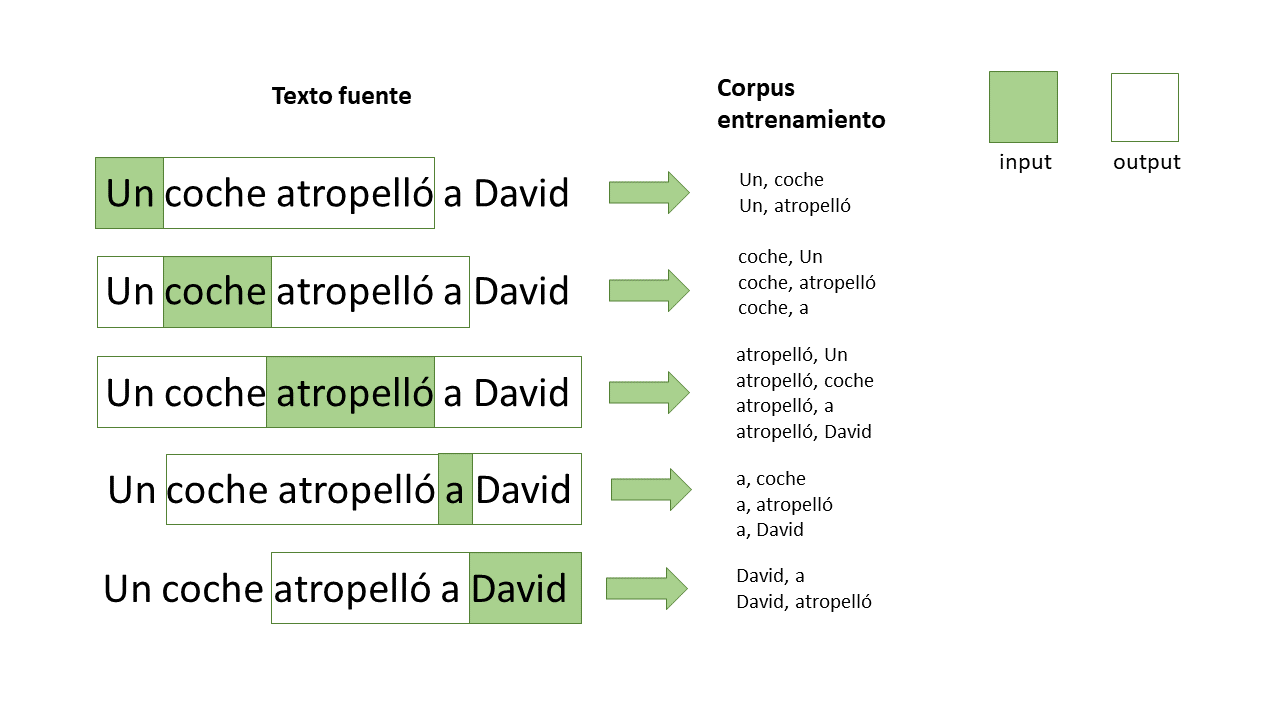
\includegraphics[scale=0.4,keepaspectratio]{imagenes/ex_skipgram.png} %[width=4cm,,keepaspectratio]
	\captionof{figure}{Ejemplo algoritmo skpigram}	
\end{center}

La principal desventaja de utilizar el corpus generado en la figura 2.2 es que, al buscar una palabra del vocabulario como salida del modelo, es necesario indicar una probabilidad para cada elemento del vocabulario. Esto puede ser computacionalmente muy costoso m�s a�n si tenemos en cuenta que pueden existir millones de t�rminos en un �nico vocabulario. Por ello, en lugar de intentar predecir la palabra ``vecina'' dado un t�rmino de entrada, se modifica el enfoque y se realiza la predicci�n de la probabilidad de que dos palabras sean ``vecinas'' dados dos t�rminos de entrada. De este modo, el corpus de la figura 2.2 se ver� modificado y se tendr�n ambas palabras como entrada al modelo de predicci�n y, como etiqueta, se utiliza un ``1'' habitualmente para representar los t�rminos vecinos y un ``0'' para el resto de casos. Sin embargo, en la figura 2.2 todos los ejemplos son vecinos y, por tanto, el corpus solo tendr�a ejemplos de este tipo para el entrenamiento. Para un correcto funcionamiento del clasificador, es necesario presentar patrones de entrada que no sean vecinos y, para ello, se utiliza el procedimiento de \textit{negative sampling} o muestreo negativo. En este proceso, se muestrean varios ejemplos negativos (t�rminos que no sean vecinos) para cada caso utilizando el corpus existente. Por tanto, el corpus de la figura 2.2 se completar�a con ejemplos negativos de t�rminos de otros documentos del corpus, por ejemplo, en la primera iteraci�n se podr�a a�adir los patrones \textit{(Un, saltar, 0)} o \textit{(Un, violeta, 0)} como ejemplos negativos. Esta t�cnica aplicada junto con el m�todo \textit{skipgram}, constituyen los dos elementos m�s importantes en el proceso de entrenamiento de \textit{word2vec}.

Previo al entrenamiento del algoritmo, se establece un tama�o de vocabulario, por ejemplo, 10.000 t�rminos. Tras esto, se crean dos matrices: la matriz \textit{embedding} y la matriz de contexto. Estas dos matrices tendr�n tama�o $[vxe]$ done $v$ corresponde al tama�o del vocabulario y $e$ al n�mero de elementos que contendr� el vector final de n�meros reales con el que se codificar� el texto. Estas dos matrices almacenan las palabras del vocabulario y se inicializan sus vectores asociados con valores aleatorios para comenzar el proceso de entrenamiento.

Para comenzar el entrenamiento, se toma un ejemplo positivo y sus ejemplos negativos asociados. Para el primer caso de la figura 2.2, se tomar�a el ejemplo positivo \textit{(Un, coche, 1)} y sus ejemplos negativos asociados \textit{(Un, saltar, 0), (Un, violeta, 0)}. De este modo, se tendr�an cuatro palabras: la entrada \textit{Un} y \textit{coche, saltar, violeta} como contexto. En el siguiente paso, se busca la palabra de entrada en la matriz de \textit{embedding} y el resto en la matriz de contexto. A continuaci�n, se realiza el producto escalar para los 3 vectores y se compara el resultado con las etiquetas \textit{(1, 0, 0)} para este caso. En la primera iteraci�n, al estar inicializadas las matrices con valores aleatorios, los resultados no coincidir�n con las etiquetas, por tanto, es necesario actualizar las matrices de \textit{embedding} y contexto seg�n el error cometido. Para este proceso, se utiliza el m�todo de descenso de gradiente estoc�tico \cite{Bengio2003}. Este proceso completo se repite para todos los patrones de entrada durante un n�mero de iteraciones que, como resultado, generar� la matriz de \textit{embedding} con los vectores de n�meros reales asociados a cada t�rmino del vocabulario.

La matriz de \textit{embedding} resultante del proceso de entrenamiento contendr�, por tanto, un vector num�rico para cada t�rmino que exista dentro del vocabulario. Por ejemplo, si existiera la palabra ``banco'' dentro del corpus de entrenamiento, esta matriz contendr�a un vector num�rico que identificar�a esta palabra y su relaci�n sem�ntica con el resto de t�rminos que conforman el corpus. Sin embargo, debido a la ambig�edad del lenguaje, este t�rmino puede tener m�s de un significado dependiendo del contexto, por ejemplo, se podr�a encontrar el t�rmino dentro de los siguientes documentos:

	\textit{``He ido al banco a ingresar dinero''}
	
	\textit{``Me he sentado en el banco del parque''}
	
Pese a que el significado del t�rmino es distinto, el algoritmo \textit{word2vec} representar�a la palabra con el mismo vector. Para abordar este problema, surgen los m�todos de \textit{word-embeddings} contextualizados. En este tipo de m�todos, en lugar de utilizar un vector fijo para cada t�rmino, se observa el contexto en el que se utiliza para asignar un vector con el que codificar la palabra. Dentro de estos m�todos destacan ELMo \cite{Matthew2018} y BERT \cite{Jacob2019} que ha alcanzado los mejores resultados hasta la fecha para numerosas tareas relacionadas con el procesado del lenguaje.


\subsection{Clasificaci�n}
\label{sec:Ejemplo_subSeccion} 
\noindent Como ya se introdujo en apartados anteriores, la clasificaci�n autom�tica de documentos se puede entender como aquella tarea en la que un documento, o una parte del mismo, es etiquetado como perteneciente a un determinado conjunto, grupo o categor�a predeterminada.

Los m�todos de clasificaci�n supervisados utilizan un conjunto de documentos de ejemplo para cada una de las categor�as que presenta la variable objetivo (a clasificar). Estos algoritmos, realizan una etapa de entrenamiento donde se presentan los patrones de ejemplo de modo que ante futuros patrones, el algoritmo ser� capaz de clasificar en alguna de las clases contenidas en el conjunto de ejemplo. Dentro de este proceso, existen muchas variables que influir�n en los resultados del sistema como el tama�o del conjunto de ejemplo, la elecci�n del algoritmo de clasificaci�n o los par�metros de inicializaci�n del mismo.

Existen numerosos tipos de algoritmos de clasificaci�n, a continuaci�n se indican los m�s importantes para clasificaci�n textual:

\begin{itemize}
	\itemsep0em 
	\item Naive Bayes \cite[Capitulo~3]{Jurafsky}: Est� basado en la teor�a de la decisi�n de Bayes: la teor�a de las probabilidades condicionadas. Por tanto, el problema de la clasificaci�n se reduce al c�lculo de las probabilidades a posteriori de una clase dado un documento.
	\item Arboles de decisi�n \cite{Leo2001}: Se trata de un m�todo que a trav�s de un proceso recursivo de las los atributos de entrada, realiza una representaci�n para clasificar el conjunto de datos presentado.
	\item M�quinas de vectores de soporte (``Support Vector Machine'', SVM) \cite{Corinna1995}: Estos algoritmos pretenden encontrar una hipersuperficie de separaci�n entre clases dentro del espacio de representaci�n.
	\item Redes Neuronales \cite{Goodfellow-et-al-2016}: Son un modelo computacional compuesto por elementos ("neuronas") interconectados entre s� que aplican una transformaci�n a los datos para producir una salida. Es posible entrenar una red neuronal para que dada una entrada determinada (un vector de representaci�n) produzca una salida deseada (la categor�a a la que corresponde ese documento). Dentro de este tipo de algoritmos, destacan las ``redes neuronales profundas'' (\textit{deep learning}) que proveen de una herramienta muy poderosa a�adiendo m�s capas de neuronas que permiten representar funciones de mayor complejidad. Este tipo de t�cnicas alcanza los mejores resultados hasta la fecha en tareas como el procesado de imagen \cite{Mingxing2019} o el procesado de textos \cite{Jacob2019}.
	\item KNN (K-Nearest Neighbour) \cite{Gongde2003}: Este algoritmo se basa en la aplicaci�n de una m�trica que establezca la similitud entre un documento que se quiere clasificar y cada uno de los documentos de entrenamiento. La clase o categor�a que se asigna al documento ser�a la categor�a del documento m�s cercano seg�n la m�trica establecida.
\end{itemize}

%Random forest (Breiman, 2001) is an ensemble of unpruned classification or regression trees, induced from
%bootstrap samples of the training data, using random feature selection in the tree induction process. Prediction is made by aggregating (majority vote for classification or averaging for regression) the predictions of
%the ensemble. Random forest generally exhibits a substantial performance improvement over the single tree
%classifier such as CART and C4.5. It yields generalization error rate that compares favorably to Adaboost,
%yet is more robust to noise. However, similar to most classifiers, RF can also suffer from the curse of learning from an extremely imbalanced training data set. As it is constructed to minimize the overall error rate, it
%will tend to focus more on the prediction accuracy of the majority class, which often results in poor accuracy
%for the minority class. To alleviate the problem, we propose two solutions: balanced random forest (BRF)
%and weighted random forest (WRF).

\section{Detecci�n de lenguaje o discurso del odio (\textbf{\textit{hate speech detection}}) }
\label{sec:Ejemplo_seccion}
La detecci�n del lenguaje machista o sexista est� muy relacionada con la detecci�n del lenguaje o discurso del odio en redes sociales. Existen numerosos trabajos donde se intenta detectar distintos tipos de lenguaje del odio, entre ellos el sexismo \cite{Watanabe2018,WaseemHovy2016,Georgios2018,Badjatiya2017,Zimmerman2018,Park2017,Waseem2016}. El lenguaje del odio se refiere al uso de lenguaje agresivo, violento u ofensivo hacia un grupo espec�fico de personas que comparten una propiedad en com�n, sea esta propiedad su g�nero, su raza, sus creencias o su religi�n \cite{Davidson2017}. Atendiendo a esta definici�n, se puede considerar la detecci�n del machismo como un caso particular del discurso del odio. Por ello, es muy interesante realizar una evaluaci�n de los trabajos realizados en esta l�nea de investigaci�n.

La detecci�n del lenguaje del odio es una linea de investigaci�n muy actual, datando el primer estudio evaluado en el a�o 2012 \cite{Xiang2012}. En este articulo se emplea un modelo de detecci�n de temas o categor�as (\textit{topic modelling}) que explota la concurrencia de palabras para la creaci�n de atributos o \textit{features} que alimentar�n un algoritmo de clasificaci�n de aprendizaje de m�quina o \textit{machine learning}. En la mayor�a de trabajos previos se empleaban soluciones basadas en patrones para la clasificaci�n de tweets. Utilizando estos m�todos, el uso de expresiones coloquiales y soeces en redes sociales hace m�s complicado establecer las fronteras entre el uso de lenguaje ofensivo que no tiene como objetivo despreciar a ning�n grupo de personas y el lenguaje del odio \cite{Davidson2017}. De este modo, este art�culo supone un paso muy importante hacia la automatizaci�n y a los sistemas basados en algoritmos de \textit{machine learning}.

Durante los �ltimos tres a�os, se han sucedido diferentes art�culos en la tem�tica aumentando considerablemente la producci�n cient�fica en este campo. En \cite{WaseemHovy2016} se aporta el primer corpus de referencia anotado que se utilizar� posteriormente en \cite{Waseem2016,Georgios2018,Badjatiya2017,Zimmerman2018,Park2017}. Est� compuesto por 16.000 \textit{tweets} etiquetados en mensajes sexistas, racistas o sin contenido ofensivo. En este primer trabajo, se sientan las bases de las soluciones aplicadas en el resto de art�culos, se utilizan atributos como los \textit{unigramas, bigramas, trigramas} y \textit{cuatri-gramas} y un algoritmo de regresi�n log�stica para la clasificaci�n.

En el art�culo desarrollado por el mismo autor \cite{Waseem2016} se propone una soluci�n similar pero se ampl�a el corpus en 4033 \textit{tweets} y se utiliza una plataforma de \textit{crowdsourcing} para anotar los mensajes, lo que introduce m�s diversidad en los criterios del etiquetado. Seg�n los autores, el empeoramiento de los resultados puede deberse al posible sesgo que se produce en \cite{WaseemHovy2016}, ya que los \textit{tweets} fueron etiquetados por los autores �nicamente.

En el resto de art�culos que eval�an su propuesta utilizando el corpus desarrollado por \cite{Waseem2016}, se utilizan redes neuronales en la etapa de clasificaci�n y, en algunos, en la etapa de preprocesamiento. En la soluci�n propuesta por \cite{Zimmerman2018} se aplican redes neuronales convolucionales (\textit{CNN, Convolutional Neural Network}) para codificar el texto y extraer los atributos que se utilizar�n para el clasificador final, basado tambi�n en CNNs. Esta t�cnica permite tener en cuenta la posici�n de la palabra (su contexto) para extraer los atributos de cada \textit{tweet}. Esta misma idea junto con el uso de redes neuronales recurrentes (\textit{RNN, Recurrent Neural Network}) se utiliza en \cite{Badjatiya2017} para obtener los atributos en la etapa de procesamiento. En ambos art�culos se consiguen mejorar los resultados alcanzados por \cite{Waseem2016} lo que afianza el uso de t�cnicas basadas en redes neuronales en el procesado del lenguaje.

Una idea interesante es el uso de atributos como la tendencia al racismo o al sexismo sirvi�ndose del historial de los usuarios. En \cite{Georgios2018} se demuestra como el uso de este tipo de atributos mejora notablemente los resultados. Esta misma idea se utiliza en \cite{Chatzakouy2017} donde se detectan cuentas agresivas estudiando al usuario y su red de seguidores.

En todos los art�culos revisados anteriormente, se trata el problema como una clasificaci�n m�ltiple donde el texto se puede clasificar seg�n las etiquetas racismo, sexismo o ninguno. Sin embargo, se podr�a resolver el problema con un doble clasificador, el primero detecta si el texto contiene lenguaje abusivo o no y el segundo realizar�a la tarea de clasificar en contenido sexista o racista \cite{Park2017}.

Un desaf�o importante en la detecci�n del lenguaje del odio en redes sociales es la separaci�n entre el lenguaje ofensivo y el lenguaje que incita o promueve el odio. Davidson \cite{Davidson2017} aporta un corpus etiquetado de 25.000 \textit{tweets} para diferenciar entre estos 2 tipos de lenguaje. En su trabajo, se propone un modelo similar a \cite{Waseem2016} donde se ponen de manifiesto las dificultades de esta soluci�n para considerar el contexto de las palabras. De este modo, si se utilizan palabras que pueden expresar odio (por ejemplo, "\textit{gay}") en un contexto positivo, hay muchas probabilidades de que el sistema detecte odio en el texto. Los resultados ser�n mejorados posteriormente en \cite{Watanabe2018} donde se ampliar� el n�mero de \textit{features} y se utilizar� un algoritmo basado en �rboles de decisi�n para la tarea de clasificaci�n.


\section{Detecci�n de la misoginia}
\label{sec:Ejemplo_seccion}
La misoginia se define seg�n la RAE como \textit{``Aversi�n a las mujeres''} \cite{MisoginiaRAE}. El machismo, sin embargo, se define como ``Actitud de prepotencia de los varones respecto de las mujeres'' o ``forma de sexismo caracterizada por la prevalencia del var�n'' \cite{MachismoRAE}. Si bien estos dos t�rminos tienen matices distintos, tienen como denominador com�n la discriminaci�n de las mujeres debido a su sexo. De hecho, existen trabajos donde se expone que la misoginia se manifiesta ling��sticamente mediante la exclusi�n, discriminaci�n, hostilidad, trato de violencia objetificaci�n o cosificaci�n sexual \cite{Anzovino2018,Fersini2018}. Muchas de estas se�ales textuales de misoginia ser�an aplicables del mismo modo al machismo \cite{Garazi2014,Giraldo1972}. 

Durante este �ltimo a�o, se ha llevado a cabo la competici�n IberEval 2018 donde una de las tareas era la detecci�n autom�tica de la misoginia \cite{AMI2018} (AMI, \textit{``Automatic Misogyny Identification''}). En esta tarea se propone la labor de identificar la misoginia en \textit{tweets} en espa�ol e ingl�s. En total, participaron once equipos de cinco pa�ses distintos para la detecci�n en ingl�s, mientras que para la detecci�n en castellano participaron un total de ocho equipos \cite{AMIOverview2018}. Los art�culos publicados para esta tarea en castellano resultan de gran inter�s, pues guarda una relaci�n importante con el presente trabajo.

Para la tarea de clasificaci�n, la mayor�a de los equipos utilizaron M�quinas de Vectores de Soporte (SVM, \textit{Suppor Vector Machines}) y m�todos combinados de aprendizaje (EoC, \textit{Ensemble of Classifiers}). Las t�cnicas basadas en SVMs fueron utilizadas por \cite{Canos2018,Wahyu2018,Victor2018} mientras que los equipos \cite{Ahluwalia2018,Shushkevich2018,Frenda2018,Liu2018} aplicaron t�cnicas EoC.

Las soluciones aportadas por \cite{Canos2018,Wahyu2018} obtuvieron la mejor tasa de acierto para la detecci�n de la misoginia en castellano. El modelo propuesto por \cite{Canos2018} utiliza \textit{features} basadas en la vectorizaci�n de cada tweet, utilizando la medida tf-idf (\textit{term frequency - Inverse document frequency}). Posteriormente, se emplea un modelo SVM con n�cleo lineal para la etapa de clasificaci�n. Esta soluci�n tan sencilla alcanza los mejores resultados para \textit{tweets} en castellano, pero empeora considerablemente para \textit{tweets} en ingl�s.

Una idea interesante, explorada en \cite{Wahyu2018}, es el uso de un l�xico auxiliar que contenga palabras que se encuentren con frecuencia en textos sexistas. Este l�xico fue desarrollado en un trabajo italiano \cite{Mauro2016}. En dicho estudio, se utiliza como clasificador un modelo basado en SVM con n�cleo lineal para el castellano y n�cleo radial para el ingl�s. En este caso, se alcanza la m�xima tasa de acierto en ingl�s y en espa�ol.

\cite{Goenaga2018} fue uno de los pocos trabajos donde se exploraron soluciones basadas en redes neuronales. En este trabajo se utilizan redes neuronales recurrentes (\textit{Recurrent Neural Network, RNN}) como sistema de clasificaci�n realizando previamente un preprocesado basado en \textit{word embeddings} que permite codificar las palabras o t�rminos mediante n�meros reales. Pese a que este tipo de t�cnicas han mostrado su eficacia en tareas relacionadas con el procesado de texto \cite{Jacob2019}, esta soluci�n queda lejos de los mejores resultados alcanzados en la competici�n.

\subsection{Corpus disponibles}
\label{sec:Ejemplo_subSeccion} 
A continuaci�n se citan algunos corpus que pueden ser utilizados para la detecci�n de lenguaje del odio en textos:
\begin{itemize}
	\itemsep0em 
	\item IberEval 2018 Automatic Misogyny Identification \cite{AMIOverview2018}: Se trata de un corpus etiquetado que contiene campos que denotan si el texto contenido en un tweet tiene un componente sexista. Fue recogido entre el 20-07-2018 y 30-11-2017 donde se recogieron 83 millones de tweets en ingl�s y 72 millones en castellano. Para el proceso de etiquetado se utilizadon dos pasos: en el primero dos anotadores etiquetaban el conjunto y en el segundo se utiliz� una plataforma de crowdsourcing. Finalmente, se etiquetaron 3521 tweets en ingl�s y 3307 en espa�ol para la fase de entrenamiento. En cuanto al conjunto de test, se compartieron 831 tweets en espa�ol y 726 en ingl�s.
	\item Corpus etiquetado \cite{WaseemHovy2016}: Est� compuesto por \textit{tweets} etiquetados para mensajes sexistas, racistas o sin contenido ofensivo. Se trata de un conjunto de datos recolectado durante dos meses y compuesto por 136.052 de los cuales se etiquetaron 16.614. De los tweets etiquetados, 3.383 contienen mensajes machistas, 1972 contienen expresiones racistas y  11.559 mensajes libres de contenido ofensivo. 
\end{itemize}
 

%%%%%%%%%%%%%%%%%%%%%%%%%%%%%%%%%%%%%%%%%%%%%%%%%%%
%%% Herramientas utilizadas
%%%%%%%%%%%%%%%%%%%%%%%%%%%%%%%%%%%%%%%%%%%%%%%%%%%

\chapter{Herramientas utilizadas}
\fancyhead[RE]{\textsc{CAP�TULO} \thechapter. Herramientas utilizadas}
\label{ch:Herramientas}

\noindent En este cap�tulo se describen en profundidad las distintas herramientas evaluadas para la creaci�n del sistema propuesto. Adem�s, se exponen los motivos por los que se han elegido frente a otras alternativas disponibles.

\section{Crawler}
\label{sec:Ejemplo_seccion}
\subsection{Amazon Web Services}{}
\label{sec:Ejemplo_seccion}
\noindent AWS es una creciente unidad dentro la compa��a Amazon.com que ofrece una importante variedad de soluciones de Cloud Computing a empresas tanto PYMES como grandes organizaciones a trav�s de su infraestructura interna siendo la marca m�s utilizada actualmente en el mercado de la nube con casi un 40\% de cuota de mercado \cite{AWScuota}. Amazon ofrece unos servicios en la nube p�blica mediante una tarificaci�n de precios en funci�n del tiempo de uso, anchos de banda consumidos, etc. Por lo tanto, su gran ventaja competitiva es ofrecer unos recursos de infraestructura y plataforma poco asumibles a la mayor�a de empresas para el periodo que se requiera. 

Los clientes de AWS tan s�lo deben pagar lo que usen del servicio, de esta manera, obtener unos potentes servidores con una plataforma determinada, un espacio de almacenamiento o una gran base de datos supone la adquisici�n de un hardware que no se aproveche todo el tiempo, que tan s�lo interese para un periodo determinado y satisfacer una necesidad puntual, prescindiendo de importantes inversiones en infraestructura. Orientado a empresas, se adapta con total flexibilidad y escalabilidad a las necesidades de Cloud que tenga el cliente, mediante un acuerdo de nivel de servicio, se especifica el nivel de compromiso del servicio, disponibilidad y ofrece un punto de confianza que otros proveedores de nube p�blica no proporcionan, dato que le da ventaja frente a sus competidores.

Dado que ha sido pionero en el sector y posee una gran cantidad de desarrolladores que trabajan para mejorar el servicio, desde su publicaci�n en 2006, ha sido l�der en el sector por delante de Google App Engine, Azure de Microsoft, Alibaba, etc \cite{AWScuota}. Siempre ha ido un paso por delante y le ha permitido innovar en el sector y ofrecer unos precios muy competitivos, soluciones para todos los gustos e importantes acuerdos con Microsoft, IBM y HP como estrategias de marketing para ofrecer software y plataformas propietarias (adem�s de software libre que fue lo primero que se ofrec�a con plataformas Linux) en sus im�genes de m�quinas virtuales. En la siguiente figura se puede ver un resumen de los servicios de AWS:

\begin{center}
	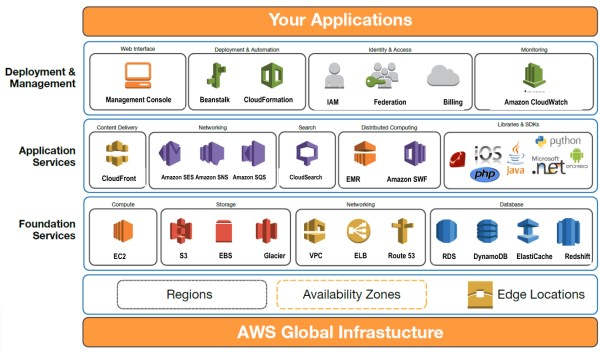
\includegraphics[width=0.9\textwidth]{imagenes/aws_services.jpg} %[width=4cm,,keepaspectratio]
\end{center}


Los diferentes servicios de AWS se incrementan con el paso del tiempo, siendo EC2, S3 y Lambda los que m�s peso tienen en el presente proyecto:

\begin{itemize}
	\itemsep0em 
	\item Amazon Elastic Compute Cloud (EC2): proporciona servidores virtuales escalables. Proporciona las capacidades de Cloud Computing a sus clientes de manera que permite una configuraci�n y administraci�n de las capacidades de m�quinas virtuales que se solicitan a la nube, pudiendo pagar tan s�lo el tiempo de computaci�n. Actualmente existen numerosos tipos de instancias con caracter�sticas hardware distintas seg�n los requisitos del usuario.
	\item Amazon Simple Storage Service (S3): proporciona un Web Service basado en el almacenamiento online para aplicaciones. Este almacenamiento en Internet proporciona una simple interfaz web, como su nombre indica, que puede ser usada para almacenar grandes cantidades de datos en cualquier momento desde cualquier sitio, dando acceso confiable y seguro con SLA, altamente escalable, r�pido y barato en la infraestructura de Amazon. F�sicamente, los datos est�n distribuidos por los Data Center de Amazon, pero es algo que permanece ajeno al cliente y de lo que no debe preocuparse (escalabilidad). Su integraci�n con EC2 es esencial para que las im�genes de m�quinas virtuales puedan trabajar con datos y objetos almacenados en S3 y tener un espacio donde los desarrolladores puedan trabajar c�modamente incluso poder solicitar m�s espacio temporal para las m�quinas o disponer de varios ?buckets? donde compartir datos entre instancias.
	\item AWS Lambda: se trata de un servicio de computaci�n sin servidor. Este servicio permite ejecutar c�digo sin aprovisionar ni administrar servidores, pagando �nicamente por el tiempo de c�mputo que se consuma. De este modo, este servicio permite que se AWS quien se encargue de la administraci�n de las m�quinas y el usuario �nicamente trabaje en el c�digo que se ejecuta.
\end{itemize}

La segunda plataforma de cloud computing m�s importante a nivel mundial es Azure, propiedad de la empresa Microsoft. En este caso, no se ha elegido Microsoft Azure porque ya se contaba con un conocimiento previo en el uso de los servicios de AWS. Adem�s, AWS cuenta con servicios de computaci�n serverless, como AWS Lambda, muy �tiles para la realizaci�n del crawler. 

\subsection{Twitter API y rtweet}{}
\label{sec:Ejemplo_seccion}
\noindent Twitter proporciona m�ltiples APIs para facilitar el acceso a los datos de su plataforma. De todas ellas, la necesaria para crear el corpus objetivo ser�a el API REST de Twitter. En concreto, es necesario utilizar la funcionalidad Tweet Search que permite realizar b�squedas de los tweets generados en la plataforma seg�n distintos par�metros de b�squeda.

Dentro del API existen 3 tipos de cuenta seg�n la cantidad de informaci�n disponible para consulta: Standard Search, Premium Search y Enterprise Search. De todas ellas, solamente la primera es gratuita por lo que ser� la utilizada durante el proceso de generaci�n del corpus. Es importante se�alar que este tipo de b�squeda presenta algunas limitaciones. Las dos m�s importantes ser�an la existencia de una ventana temporal de consulta limitada a 7 d�as anteriores y, por otra parte, la limitaci�n de descarga de tweets a 18.000 cada 15 minutos.

Para recopilar la informaci�n de Twitter, se ha utilizado la herramienta rtweet \cite{rtweet-package}. Se trata de un cliente del lenguaje de programaci�n R para acceder al API de Twitter. Este paquete facilita mucho las tareas habituales como la b�squeda de tweets.

Existen varias alternativas a rtweet como tweetpy para el lenguaje de programaci�n Python o twitteR. Se ha optado por rtweet porque ambas alternativas est�n m�s desactualizadas y son proyectos mucho m�s inactivos


\section{Preprocesado y tokenizaci�n}
\label{sec:Ejemplo_seccion}

\noindent En la etapa inicial para la clasificaci�n de textos, se aplican distintas t�cnicas que permitan Extraer los atributos o \textit{features} necesarias para realizar una representaci�n fiel del texto y que permita la utilizaci�n de un algoritmo de clasificaci�n. Existen multitud de procedimientos aplicables en esta etapa como la tokenizaci�n, el reconocimiento de entidades nombradas, el etiquetado sint�ctico y morfol�gico:

\begin{itemize}
	\itemsep0em 
	\item Tokenizaci�n: Permite separar cada palabra o s�mbolo del corpus en unidades independientes (como palabras) que pueden ser almacenadas para su posterior procesado.
	\item Reconocimiento de entidades nombradas: Tarea que permite clasificar en categor�as predefinidas, como personas, organizaciones, lugares, expresiones de tiempo y cantidades.
	\item Etiquetado sint�ctico: Proceso en el que se busca sobre el espacio de todas las posibles combinaciones de las reglas gramaticales definidas para encontrar la estructura de una oraci�n.
	\item Etiquetado morfol�gico: En este proceso se le asigna a cada palabra su funci�n dentro del corpus utilizado. Normalmente, se utilizan 8 etiquetas distintas en la mayor�a de los idiomas utilizados en Europa: nombre, verbo, pronombre, preposici�n, adverbio, conjunci�n, part�cula y articulo.
\end{itemize}

Para aplicar este tipo de t�cnicas, existen gran cantidad de proyectos o librer�as de computaci�n disponibles. Algunas de las m�s utilizadas son las siguientes:

\begin{itemize}
	\itemsep0em 
	\item Freeling: Es una librer�a que soporta el lenguaje espa�ol y se utiliza en \cite{Frenda2018}. Pese a que tiene mucha de las caracter�sticas que se necesitan, tiene una menor comunidad y est� menos extendido que algunas del resto de las herramientas.
	\item Stanford Parser: Se trata de una librer�a desarrollada por el grupo de trabajo de NLP de la universidad de Stanford.
	\item TweetNLP: Librer�a desarrollada espec�ficamente para le procesado de tweets. Su uso no est� muy extendido.
	\item Spacy: Se utiliza en \cite{Waseem2016} y permite aplicar las t�cnicas de procesado de un modo eficiente.
	\item NLTK: Se trata de la librer�a m�s extendida para el preprocesamiento, se utiliza en \cite{Zimmerman2018,Davidson2017,Frenda2018}.
\end{itemize}

De todas las herramientas listadas, se ha optado por la librer�a NLTK. Se trata de una librer�a muy extendida que cuenta con una gran comunidad y permite un desarrollo muy �gil. Algunas librer�as como Freeling o Stanford Parser requieren varias dependencias para poder ser utilizadas.

La mejor alternativa a NLTK considerada ser�a Spacy. Su uso est� aumentando y su funcionamiento es muy similar ya que ambas est�n desarrolladas en Python. Se ha optado por NLTK porque a�n sigue siendo m�s utilizada.

\subsection{NLTK: Natural Language Toolkit}{}
\label{sec:Ejemplo_seccion}
\noindent NLTK es una librer�a que define una infraestructura en la que crear programas para el procesado del lenguaje natural (NLP, ``Natural language processing'') en ``Python''. Provee la estructura b�sica para representar datos relevantes para el procesado del lenguaje natural, interfaces para realizar tareas como el etiquetado del discurso (POS, ``part-of-speech tagging''), etiquetado sint�ctico y clasificaci�n de texto \cite{NLTKweb}.

Esta librer�a fue desarrollada originalmente en el a�o 2001 como parte de un curso de ling��stica computacional en la universidad de Pennsylvania. Desde entonces, ha sido desarrollado y mejorado por distintos contribuidores al tratarse de un proyecto libre. Actualmente, NLTK es utilizado en gran cantidad de investigaciones y supone un est�ndar muy importante para realizar tareas relacionadas con NLP. Est� compuesto por una cantidad importante de m�dulos que pueden ser invocados desde un programa escrito en Python. En la siguiente figura se recogen los m�s importantes \todo{Explicar con m�s detalle los m�dulos que utilice en el trabajo} \cite{Bird2009}:

(LA IMAGEN PROVOCA QUE SE DESCUADRE EL DOCUMENTO)

\begin{center}
	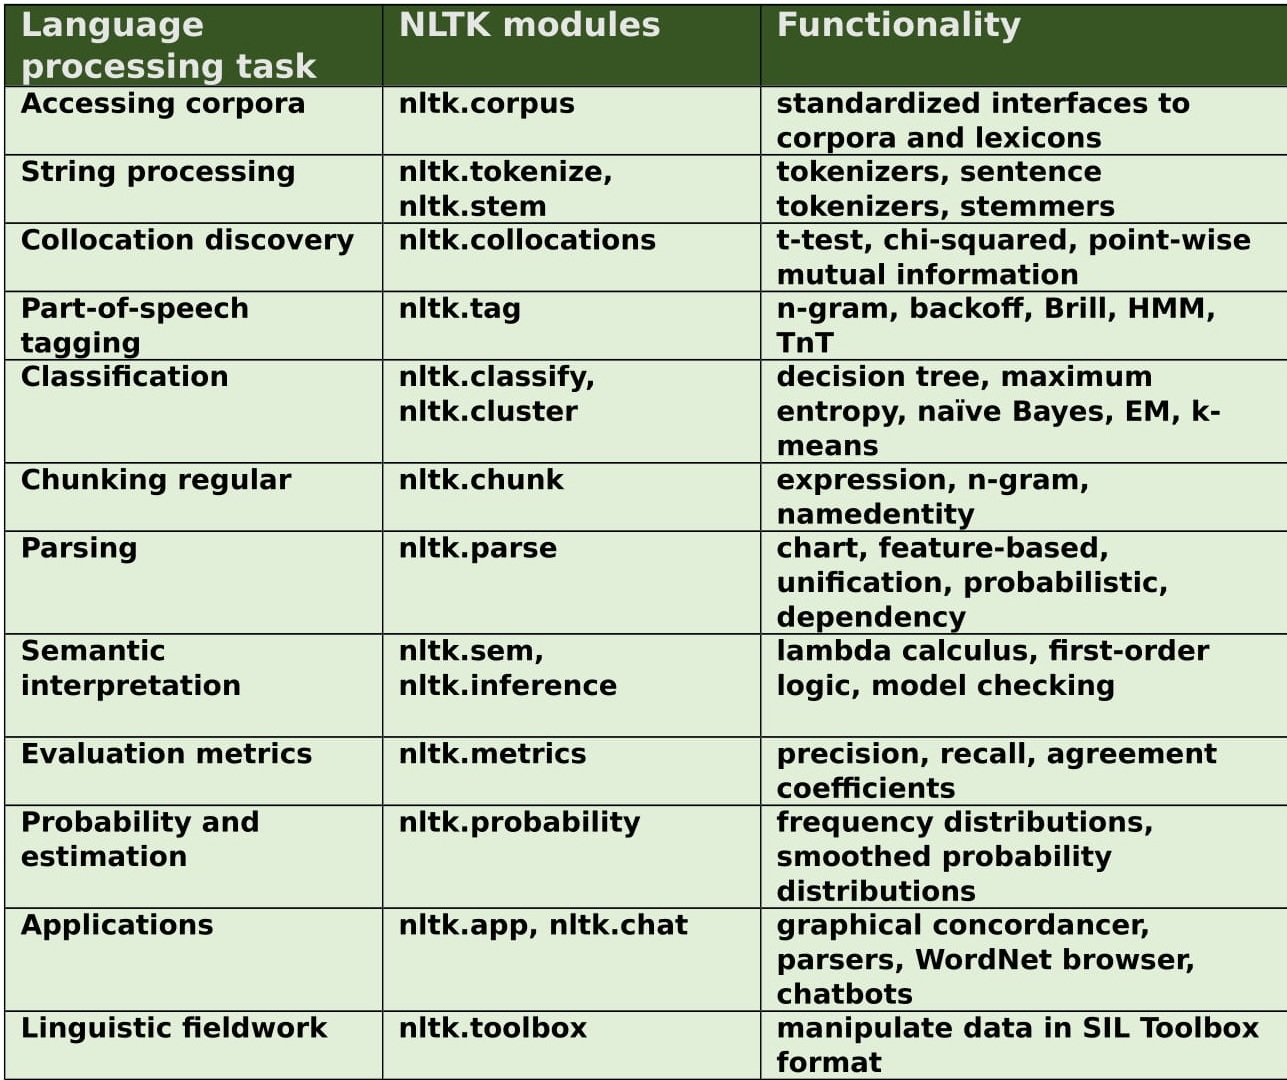
\includegraphics[width=0.9\textwidth]{imagenes/NLTK_modules-1.jpg} %[width=4cm,,keepaspectratio]
\end{center}

\section{Scikit-learn}
\label{sec:Ejemplo_seccion}

\noindent Tal y como se ha ido introduciendo, el objetivo final del presente trabajo es la detecci�n del lenguaje machista en las redes sociales. Este problema se puede modelar como una clasificaci�n de documentos en los que en este caso se asignar� una categor�a a cada uno de los mensajes que conforman el corpus. 

En la actualidad, la mayor�a de trabajos llevan a cabo esta tarea mediante algoritmos o t�nicas de aprendizaje supervisado \cite{Zimmerman2018,Davidson2017,AMIOverview2018}. Para el desarrollo de este tipo de m�todos se utilizar� la librer�a ``scikit-learn'' muy utilizada en proyectos de clasificaci�n de documentos \cite{Ahluwalia2018}.

Scikit-learn \cite{Pedregosa2011}  es un proyecto que provee una librer�a de aprendizaje de m�quina para el entorno de programaci�n ``Python''. El objetivo principal del proyecto es establecer un conjunto de herramientas dentro de un entorno de programaci�n que sea accesible a usuarios no expertos. Esta librer�a incluye algoritmos cl�sicos de aprendizaje de m�quina, herramientas para la selecci�n, evaluaci�n de modelos y preprocesado.

Todo los modelos de aprendizaje supervisados o funciones auxiliares relacionadas con el procesado de datos utilizados en el presente trabajo est�n implementados o han sido desarrollados con ayuda de funciones disponibles en la librer�a scikit-learn.

Todos los objetos dentro de la librer�a comparten un API b�sica compuesta por 3 interfaces complementarias: ``estimators'' que permiten construir y ajustar modelos, ``predictors'' para realizar predicciones y ``transformers'' que permiten realizar conversiones a los datos.

\subsection{``Estimators''}
\label{sec:Ejemplo_subSeccion}

\noindent La interfaz ``estimator'' define objetos y provee de un m�todo ``fit'' para ajustar un modelo a los datos de entrenamiento. Todos los algoritmos supervisados y no supervisados implementados en la librer�a son tratados como objetos implementando esta interfaz. Otro tipo de tareas relacionadas con el aprendizaje de m�quina como la selecci�n de atributos o m�todos para la reducci�n de la dimensionalidad tambi�n utilizan el interfaz ``estimator''.

La inicializaci�n de un ``estimator'' y el ajuste de un modelo a los datos de entrenamiento est�n diferenciados en la librer�a. Un ``estimator'' se puede inicializar un con conjunto de par�metros de entrada (por ejemplo, el par�metro C para SVM) y, posteriormente, se utiliza el m�todo ``fit'' para realizar el proceso de ajuste a los datos de entrenamiento. En el siguiente c�digo se ilustra esta funcionalidad:

\begin{lstlisting}[language=Python]
from sklearn.ensemble import RandomForestClassifier
rf = RandomForestClassifier(n_estimators=250)
rf.fit(X_train, y_train)
\end{lstlisting}

En el c�digo anterior, primero se inicializa un ``estimator'' estableciendo el argumento ``n\_estimator''. Tras esto, se realiza una llamada al m�todo ``fit'' para realizar el ajuste utilizando los datos de entrenamiento.


\subsection{``Predictors''}
\label{sec:Ejemplo_subSeccion}

\noindent La interfaz ``predictor'' extiende la funcionalidad del ``estimator'' a�adiendo el m�todo ``predict''. Este m�todo devuelve un vector de predicciones tomando como entrada una matriz con los datos de testeo. Ampliando el ejemplo anterior:

\begin{lstlisting}[language=Python]
y_pred = rf.predict(X_test)
\end{lstlisting}


\subsection{``Transformers''}
\label{sec:Ejemplo_subSeccion}

\noindent Antes de aplicar un m�todo de clasificaci�n supervisada, suele ser habitual realizar filtrados o modificaciones en los datos, para ello, ``scikit-learn'' implementa la interfaz ``transformer'' para llevar a cabo este tipo de tareas.

Esta interfaz define el m�todo ``transform'' que toma como entrada una matriz de datos y devuelve como salida una versi�n transformada de estos datos. Algunas de las transformaciones m�s comunes pueden ser la selecci�n de atributos, preprocesado o m�todos de reducci�n de dimensionalidad. Un ejemplo de preprocesado podr�a ser el estandarizado de un conjunto de datos:

\begin{lstlisting}[language=Python]
from sklearn.preprocessing import StandardScaler
scaler = StandardScaler()
scaler.fit(X_train)
X_train = scaler.transform(X_train)
\end{lstlisting}


\subsection{``Pipelines y selecci�n de modelos''}
\label{sec:Ejemplo_subSeccion}

\noindent ``Scikit-learn'' permite componer nuevos ``estimators'' utilizando otros lo que permite crear flujos de trabajo en un �nico objeto. Este tipo de tarea se puede realizar de dos modos: mediante ``Pipeline'' utilizando un modelo secuencial o mediante ``FeatureUnion''.

Los objetos ``Pipeline'' encadenan ``estimators'' en un �nico objeto. Esto permite crear flujos de trabajo siguiendo un n�mero fijo de pasos, por ejemplo: extracci�n de atributos, reducci�n de dimensionalidad, ajuste de un modelo y realizaci�n de de predicciones.

Los objetos ``FeatureUnion'' combinan multiples ``transformers'' en uno �nico y concatena los resultados. De este modo, este tipo de objeto es capaz de realizar transformaciones distintas sobre el mismo conjunto de datos o sobre una parte del mismo.

Ambos objetos pueden ser combinados para crear flujos de trabajo m�s complejos. Por ejemplo, en el siguiente c�digo se combinan dos ``Pipeline'' utilizando ``FeatureUnion'' y se a�ade un �ltimo paso ``clf'' que a�ade un clasificador.
\begin{lstlisting}[language=Python]
Pipeline([('feature-union', 
	FeatureUnion([('text-features', text_pipeline), 
	('other-features', preprocess_pipeline)])),
	('clf', LogisticRegression(penalty = ``L2'')])

\end{lstlisting}


En ``scikit-learn'' es posible realizar selecci�n de modelos mediante el meta-estimador ``GridSearchCV''. Este m�todo toma como entrada un ``estimator'' cuyos par�metros de entrada deben de ser optimizados. Para ello, se definen todos los valores que se deben de tener en cuenta en el proceso para cada par�metro de entrada.


%%%%%%%%%%%%%%%%%%%%%%%%%%%%%%%%%%%%%%%%%%%%%%%%%%%
%%% CORPUS
%%%%%%%%%%%%%%%%%%%%%%%%%%%%%%%%%%%%%%%%%%%%%%%%%%%

\chapter{MeTwo dataset (Machismo and Sexism Twitter Identification dataset)}
\fancyhead[RE]{\textsc{CAP�TULO} \thechapter. MeTwo dataset}
\label{ch:Corpus}

\noindent Este cap�tulo describe la metodolog�a utilizada para la creaci�n de un corpus en castellano que permita entrenar un sistema de detecci�n del lenguaje machista. De este modo, se ha generado un corpus utilizando como semillas un conjunto de t�rminos en castellano que, por lo general, describen actitudes machistas. Idealmente, el conjunto generado contendr� suficientes ejemplos de tweets machistas que ser�n utilizados como entrada del sistema de clasificaci�n.

Al comienzo de esta secci�n, se analiza el problema y se estudian las expresiones y t�rminos m�s empleados en textos con comportamiento machista. Se realiza una b�squeda preliminar para observar si con los t�rminos estudiados se encuentran ejemplos de textos machistas y, finalmente, se define el m�todo para extraer la informaci�n de Twitter y evaluar las caracter�sticas principales del corpus obtenido.


\section{Machismo en Twitter}
\label{sec:Met_Eval}
\noindent En este apartado, se van a definir todas las caracter�sticas que deben presentar los textos seleccionados para considerarse machistas y la lista de t�rminos o expresiones seleccionados para generar el corpus. Como primer paso, se han estudiado diversas referencias para recopilar aquellas expresiones m�s comunes que pueden conllevar a comportamientos machistas o sexistas. Posteriormente, se han identificado las expresiones m�s representativas y se han realizado diversas b�squedas para evaluar la cantidad de contenido machista que contienen dichas expresiones en Twitter. Finalmente, se han obtenido de la red social Twitter los mensajes que conten�an estas expresiones utilizando su API. Durante este estudio, solo se han considerado expresiones en castellano.

Las expresiones o t�rminos que se buscan son aquellas que, de un modo u otro, minusvaloran el papel de las mujeres en nuestra sociedad, incentivan el abuso o acoso hacia las mujeres o no les permitan expresarse libremente. Existen gran cantidad de expresiones y t�rminos que se utilizan a diario, de modo consciente o no, que minimizan el papel de la mujer en la sociedad. En \cite{TwitterSexism} la periodista Ana Isabel Bernal-Trivi�o propone, a trav�s de un hilo en su cuenta de Twitter, recopilar frases de violencia machista que las mujeres hayan escuchado o recibido en alg�n momento. Estas expresiones tienen mucho valor para el an�lisis pues un gran n�mero de mujeres aporta su experiencia personal frente al machismo. En muchos tweets se repiten t�rminos como ``ni�ata'' o ``a fregar'' que se utilizan para referirse a las mujeres de forma despectiva.

Existen refranes, dichos populares y t�picos que se utilizan diariamente y que refuerzan la idea de que las mujeres son inferiores al hombre en una tarea determinada. Por ejemplo, las expresiones ``Mujer al volante, peligro constante'' o ``�Mujer ten�a que ser!'' minusvaloran la habilidad de las mujeres para realizar una tarea espec�fica solo por ser mujeres. Otras muchas expresiones machistas se recopilaron en un trabajo realizado en un instituto de Albacete \cite{ElPais}.

Pese a que, como se ha presentado, existen gran cantidad de expresiones que conllevan actitudes machistas, ha sido necesario recoger tambi�n ciertos t�rminos m�s generales que permitan establecer una buena relaci�n entre tweets con contenido machista y aquellos que no presentan este tipo de lenguaje. Esto ser� muy importante a la hora de entrenar el sistema autom�tico de clasificaci�n. As�, partiendo de los trabajos anteriores, se han seleccionado 29 expresiones que se utilizar�n para recopilar tweets como punto de partida para la generaci�n del dataset. La tabla 1 recopila dichos t�rminos. A continuaci�n, se describen las expresiones seleccionadas.


% Please add the following required packages to your document preamble:
% \usepackage{booktabs}
\begin{table}[]
	\centering
	\begin{tabular}{@{}lll@{}}
		\toprule
		\textbf{N�mero de t�rmino} & \textbf{Texto} &  \\ \midrule
		1 & ``feminazi" &  \\
		2 & ``a la cocina" &  \\
		3 & ``a fregar" &  \\
		4 & ``marimacho" &  \\
		5 & ``ninata" &  \\
		6 & ``mujer tenias que ser" &  \\
		7 & ``las feministas" &  \\
		8 & ``en tus dias" &  \\
		9 & ``zorra" &  \\
		10 & ``como una mujer" &  \\
		11 & ``como una nina" &  \\
		12 & ``pareces una fulana" &  \\
		13 & ``pareces una puta" &  \\
		14 & ``no ha probado un hombre" &  \\
		15 & ``loca del" &  \\
		16 & ``obsesionada con el machismo" &  \\
		17 & ``para ser mujer" &  \\
		18 & ``para ser chica" &  \\
		19 & ``hombre que te aguante" &  \\
		20 & ``acabaras sola" &  \\
		21 & ``mojigata" &  \\
		22 & ``mucho feminismo pero" &  \\
		23 & ``mujer al volante" &  \\
		24 & ``las mujeres no deberian" &  \\
		25 & ``A las mujeres hay que" &  \\
		26 & ``odio a las mujeres" &  \\
		27 & ``las mujeres de hoy en dia" &  \\
		28 & ``nenaza" &  \\
		29 & ``lagartona" &  \\ \bottomrule
	\end{tabular}
	\caption{T�rminos machistas elegidos para la creaci�n del corpus}
	\label{my-label}
\end{table}


El t�rmino \textbf{``feminazi''} es una forma de relacionar, de forma claramente despectiva, al feminismo con el nazismo. De este modo, es una palabra utilizada ampliamente en redes sociales y foros de toda Espa�a que conllevan actitudes machistas. En Twitter se encuentran mensajes como:

	``\textit{Uy habl� de inventos la feminazi}''
	
	
	``\textit{Pero que violento!!! De cinco billetes, solo en uno aparece una mujer, esto es inaceptable!!! \#feminazi}''

Sin embargo, existen otros ejemplos que utilizan la expresi�n sin conllevar actitudes machistas:

``\textit{Si quieres pensar que el origen del hashtag deviene de la b�squeda del rigor hist�rico, a tope. Est�s en tu derecho, igual que yo en un texto de opini�n de valorarlo totalmente al contrario. �No te convencen mis argumentos? Intentemos debatir. �Usas "feminazi"? Te quedas solo}''

Los t�rminos \textbf{``A la cocina''} y \textbf{``A fregar''} se utilizan de modo despectivo para denigrar a la mujer o restar importancia a sus argumentos. Como en el caso del t�rmino anterior, se ha comprobado que existe una relaci�n aceptable entre mensajes machistas y aquellos que no conllevan estas actitudes. Algunos ejemplos de contenido machista:


``\textit{Hay que anunciar por megafonia que te marches a tu casa a fregar  que estas  haciendo el rid�culo .tu y las borregos}''


``\textit{De los relatos corazon... anda a la cocina a hacee algo productivo antes de seguir diciendo pavadas}''

Ejemplos que no expresan actitudes machistas:


``\textit{Me dio sed, pero me da miedo ir a la cocina}''


``\textit{Me molesta que a esta hora me d� hambre porque me da miedo ir a la cocina por algo para comer}''


Las palabras \textbf{``Marimacho''} y \textbf{``Ni�ata''}, dependiendo del contexto, se utilizan como calificativos despectivos a la mujer. Ejemplos despectivos ser�an los tweets encontrados:


``\textit{@IrantzuVarela hace unos sketches poni�ndose unas barbas postizas despeinadas. Es lo que antes se llamaba un marimacho. El igualitarismo ha hecho mucho da�o. Uno tiene que mandar y otro obedecer acr�ticamente.}''


``\textit{@carmenro\_ Mal follada y retrasada. Das pena ni�ata. Tienes un concepto muy equivocado de los andaluces y Andaluc�a. Gente como t� son las qu� no queremos en nuestra comunidad. Aqu� hay gente muy trabajadora y humilde. Envidia es lo que tienes.}''

Es importante aclarar, que en el proceso de etiquetado, el t�rmino \textbf{``Marimacho''} y \textbf{``ni�ata''} no se ha considerado machista si no se encontraba en un contexto muy claro. De forma general, \textbf{``marimacho''} se utiliza para indicar que una mujer presenta rasgos masculinos algo que, a�n pudiendo ser utilizado para expresar odio (homofobia), no se ha considerado inherentemente machista. Por otra parte, \textbf{``ni�ata''} se utiliza para indicar que una mujer es inmadura, algo que, en principio, no ser�a machista.

Las expresiones \textbf{``Mujer ten�as que ser''} y \textbf{``Las Feministas''} se utilizan para descalificar a las mujeres por el hecho de pertenecer a un colectivo. Ejemplos encontrados en Twitter son los siguientes:


``\textit{Mujer tenias que ser para dar una respuesta tan pobre}''


``\textit{@NiicoMilan Coincido eso es el verdadero machismo que tiene un respeto absoluto por la mujer m�s no lo que quieren hacer las feministas pasar por machismo.Nadie puede lastimar a una mujer}''


La expresi�n \textbf{``en tus d�as''} se utiliza como descalificativo para referirse a las mujeres por tener el periodo:



``\textit{@PriscilaTrs\_ Bb se delicia de culo no te dejar�a descansar ni cuando est�s en tus d�as mamasita rica me pasar�a d�ndole placer ma�ana tarde y noche a ese delicioso culo hasta hacerte gritar de placer}''


``\textit{Seguro era porque andabas en tus d�as. xd}''


El t�rmino \textbf{``zorra''} se utiliza continuamente en Twitter con actitudes machistas:



``\textit{zorra se puede saber pork no me sigues?}''


``\textit{Dedicado a las est�pidas feminazis que dicen que a las mujeres hay que creerles todo solo por ser mujeres.SIN PRUEBAS NO HAY DELITO.https://t.co/XNx3fk3m5K}''

Otra expresi�n que minusvalora a las mujeres considerada es \textbf{``como una mujer''} para comparar una acci�n que se realiza peor �nicamente por ser mujer:


``\textit{Un hombre sin barba es como una mujer sin nalgas}''


``\textit{\#UnMadrazoPara Cesar Gaviria, que habla como una mujer en proceso de parto.}''


Otra expresi�n similar a la anterior ser�a \textbf{``como una ni�a''}:


``\textit{No te vas a ir de aqu� sin decirme qu� sitio es ese. Y m�s te vale responder y no comportarte como una ni�a peque�a, ni�a peque�a.}''


El t�rmino \textbf{``nenaza''} se utiliza tambi�n como descalificativo en Twitter:

``\textit{A mi me ha pasado igual. Los lobos vestidos de corderos que lo mismo quieren matar fachas que lloran como una nenaza no puedo con ellos}''

``\textit{@marianorajoy ha perdido la Moncloa como una nenaza  porque no ha sabido defender como hombre y estadista a la Naci�n. Se va como los cobardes. Por la puerta de atr�s. El peor presidente de Espa�a }''

La expresi�n \textbf{``pareces una fulana''} se utiliza como descalificativo por la apariencia f�sica de las mujeres:


``\textit{Te acabo de ver en el Telenoticiasde TV3. Maquillate mejor, pareces una fulana.}''

``\textit{�L�vate esa cara que pareces una fulana!}''


Otra expresi�n muy similar a la anterior ser�a \textbf{``pareces una puta''}:


``\textit{Deja de gritar hermano, pareces una puta}''

``\textit{@emuyshondt @alcaldia\_ss @SSesTuyo podes administrar o no, porque te vibis quejan maje, mas bien pareces una puta}''


Otra expresi�n machista utilizada en Twitter es \textbf{``no ha probado un hombre''}. En este caso, se sexualiza a la mujer y se sugiere que tiene un alg�n problema o defecto por no tener relaciones con un hombre.


``\textit{que se pueda esperar de una mamerta  @ktikariza que no lee no estudia va a la provincia  tomar cerveza una millenian que no ha probado un hombre, el hambre o la guerra, estas juventud esta empecinada a decir y tener too regalado a costa de si }''

``\textit{pobre mujer, no ha probado un hombre en su vida.}''

La expresi�n \textbf{``loca del''} se utiliza de forma despectiva hacia las mujeres:

``\textit{@Madrekoraje @PhilAMellows @CasosAislados Todo los hombres tenemos que tener miedo a cruzarnos con una loca del co�o que se invente lo que le vengan en gana y por el mero hecho de tener papo haya que creerla.}''

``\textit{Odio a esta clase de feministas, loca del co�o.}''

La frase \textbf{``obsesionada con el machismo''} se utiliza para restar importancia a la denuncia del machismo que realizan las mujeres:


``\textit{T�pica obsesionada con el machismo, el patriarcado y franco. De ah� no la sacas. No evoluciona}''

``\textit{Feliz d�a de la gente tontaca obsesionada con el machismo}''

Otra expresi�n que minusvalora las habilidades de la mujer ser�a \textbf{``para ser mujer''}, pues impl�citamente da por hecho que una mujer realiza cierta acci�n peor que un hombre:


``\textit{@damita2808 @berege7 @Mariagtriana Y los ojos? Uff demasiado dureza en la mirada para ser chica...no?}''

``\textit{Para ser mujer habla bastante decente ...}''


Otra expresi�n similar a la anterior ser�a \textbf{``para ser chica''}:

``\textit{@GreatBlastG5 Mi madre mide bien para ser chica, y mi padre es de estatura media, lo de los yogures te lo dec�a a ti porque se que me mientes prro}''

``\textit{Sos un poco masculina como para ser chica, �sab�as?}''

Otra expresi�n machista utilizada en Twitter es \textbf{``hombre que te aguante''}:


``\textit{Ching�n el hombre que te aguante hasta en tus d�as. }''

``\textit{Damaris, c�sate con tu "marido (Ana)" porque no vas a encontrar un hombre que te aguante.}''


Otra expresi�n machista utilizada en Twitter es \textbf{``acabaras sola''}. En este caso, expresa que una mujer sin un hombre a su lado es una mujer ``incompleta'':


``\textit{\#SomosLaAudiencia21F  SOFIA:   � eres pat�tica, no, lo siguiente �  Deja a ALEJANDRO en paz de una vez. 
	ERES TAN PREPOTENTE que quieres ver a todos los hombres arrastr�ndose por ti.
	ACABAR�S SOLA......... TIEMPO AL TIEMPO....}''

``\textit{Nunca encontrar�s un hombre que te sorpote. Acabar�s sola, vieja, con gatos y escuchando techno}''

Otro insulto muy recurrente es \textbf{``mojigata''}:


``\textit{\#EnLaPedaNuncaFalta la mojigata persinada que con 3 tequilas encima es m�s f�cil que la tabla del 1. }''

``\textit{@Mony\_loreH Y CON ESA CARITA ME MOJIGATA QUE TIENE.....SON LAS PEORES......}''

La expresi�n \textbf{``mucho feminismo pero''} se utiliza para minusvalorar el papel del feminismo en la sociedad:

``\textit{Pues menuda hija de mierda si tienes a tu padre cargando con TODAS las tareas del hogar. Mucho feminismo, pero de compartir las labores no te ense�� nada.}''

``\textit{Mucho feminismo pero Christian Gray se las hace mojar qu� tipo hdp este pibe jajaja}''

La expresi�n \textbf{``mujer al volante''} se utiliza habitualmente para minusvalorar la capacidad de las mujeres para realizar una tarea, en este caso, conducir:


``\textit{por la prudencia con la que tomo la bajada creo que se trata de una mujer al volante }''

``\textit{No hay nada m�s peligroso que una mujer al volante con prisa . Nada, ni MALO De presidente es tan peligroso}''


La expresi�n \textbf{``las mujeres no deber�an''} sugiere que las mujeres no deben de realizar alguna tarea o acci�n por el hecho de ser mujer:


``\textit{Las mujeres no deber�an de tener ni voz ni voto, no est�n preparadas para mantener una familia menos un gobierno , son unas mantenidas}''

``\textit{Por eso es que las mujeres no deber�an tener derecho al voto}''

La frase \textbf{``A las mujeres hay que''} se utiliza habitualmente para discriminarlas o tratarlas de un modo distinto por su g�nero:


``\textit{Como dice mi pap�: ``a las mujeres hay que quererlas, no entenderlas''}''

``\textit{Hoy en d�a a las mujeres hay que tenerle un cuidado cabron. Acu�rdate que estamos en la era del chismin, la era mierdosa. Te da un abrazo y despu�s dice que le rozaste la teta. Wao! Pero si nos abrazamos! Obvio que las tetas feas esas van a rozar cabrona!}''


Otra expresi�n que suele conllevar actitudes machistas es \textbf{``odio a las mujeres''}:


``\textit{Odio a las mujeres pero me atraen sexualmente}''

``\textit{A lo que hemos llegado, lo unico que van a conseguir las feministas es el odio a las mujeres}''


La expresi�n \textbf{``las mujeres de hoy en dia''} suele expresar un sentimiento negativo hacia las mujeres solo por el hecho de ser mujer:

``\textit{Las mujeres de hoy en d�a son tan doble moral; no puedes decirle a una chica que trae el bot�n desabrochado de la blusa, por que se emperra y te tacha de pervertido, ah pero si no le dices te va peor. Tampoco es que sea un santo pero que no mamen. \#LaHubieraDejadoEnse�arTeta }''

``\textit{Se enojan las mujeres de hoy en d�a que uno les diga que parecen hombres, m�s insensibles que una piedra y m�s in�tiles en las actividades de a diario, puta no sean tan maletas prep�rense, por lo menos yo hice mi obra hoy ya se defiende en un mont�n de �reas de nada...}''

Por �ltimo, el insulto \textbf{``lagartona''} se utiliza coloquialmente para sugerir que una mujer tiene relaciones sexuales a cambio de dinero:

``\textit{@pescadosgori �Solo le quieres por el dinero? �Ay ay ay lagartona! https://t.co/7HE8PrXdDk}''

``\textit{No quiero depender de nadie. No soy una lagartona ni la zorrita de nadie, si no un hombre}''


\section{Generaci�n del corpus, ``\textit{Crawler}''}
\label{sec:Metric_Eval}

\noindent En este apartado, se especifica el proceso seguido para extraer la informaci�n deseada de Twitter. En la fase de creaci�n del corpus se ha utilizado el API de Twitter a trav�s del paquete \textit{rtweet} disponible para el lenguaje de programaci�n R. 

Las especificaciones iniciales para el desarrollo del \textit{Crawler} implican la recolecci�n diaria de 100 tweets para cada t�rmino contenido en la tabla 4.1, lo que, idealmente, har�a un total de 2900 tweets diarios. De este modo, no se superar�a el l�mite diario del API de Twitter y se recopilar�a bastante informaci�n cada d�a. Al llegar a 15000 tweets para un t�rmino, se considerar� que hay suficiente informaci�n y se dejar� de buscar los tweets que lo contengan.

Al t�rmino del proceso de \textit{crawling}, se eligir�n aleatoriamente 150 tweets para cada t�rmino. Por tanto, ser� un requisito obtener, al menos, 150 tweets para cada t�rmino para poder ser considerado.

Para esta tarea, el proceso de \textit{crawling} se ha extendido a lo largo de las fechas 1/07/2018-31/12/2018, haciendo un total de 6 meses de informaci�n. Durante este periodo, el \textit{Crawler} recolect� un total de 181792 tweets para todos los t�rminos. Para cada \textit{tweet}, el API de Twitter permite acceder a 42 atributos distintos:

\begin{itemize}
\itemsep0em 
\item status\_id: identificador �nico del tweet.             
\item created\_at: fecha de creaci�n del tweet.      
\item user\_id: identificador �nico de usuario.              
\item screen\_name: alias que el usuario utiliza para identificarse.
\item text: mensaje del tweet.                  
\item source: dispositivo/cliente utilizado para publicar el mensaje.                
\item reply\_to\_status\_id: si es una respuesta, indica el id del tweet original.    
\item reply\_to\_user\_id: si es una respuesta, indica el id del usuario original.      
\item reply\_to\_screen\_name: si es una respuesta, indica el alias del usuario original.
\item is\_quote: indica si el tweet es citado.              
\item is\_retweet: indica si el tweet es un retweet.
\item favorite\_count: conteo aproximado del n�mero de favoritos.        
\item retweet\_count: conteo aproximado del n�mero de tweets.         
\item hashtags: hastags utilizados en el tweet.              
\item symbols: s�mbolos contenidos en el mensaje.               
\item urls\_url: URLs contenidas en el texto del tweet.              
\item urls\_t.co: URLs en formato acortado.             
\item urls\_expanded\_url: URLs en formato expandido.     
\item media\_url: URLs de los elementos subidos con el tweet.             
\item media\_t.co: URLs acortadas de los elementos subidos con el tweet.           
\item media\_expanded\_url: URLs expandidas de los elementos subidos con el tweet.  
\item media\_type: tipo de elemento subido junto al tweet (por ejemplo, foto).            
\item ext\_media\_url: URLs del elemento externo adjunto al tweet.         
\item ext\_media\_t.co: URLs acortada del elemento externo adjunto al tweet.                
\item ext\_media\_expanded\_url: URLs expandidas del elemento externo adjunto al tweet.         
\item ext\_media\_type: tipo del elemento externo adjunto al tweet.        
\item mentions\_user\_id: identificadores de otros usuarios nombrados en el tweet.      
\item mentions\_screen\_name: alias de otros usuarios nombrados en el tweet.  
\item lang: idioma del tweet.                  
\item quoted\_status\_id: identificador del tweet citado.       
\item quoted\_text: texto del tweet citado.           
\item retweet\_status\_id: si es un retweet, indica el identificador del tweet original.     
\item retweet\_text: texto del retweet original.
\item place\_url: URL que representa la localidad y aporta informaci�n adicional.            
\item place\_name: nombre de la localidad.            
\item place\_full\_name: nombre de la localidad con informaci�n a�adida (por ejemplo, provincia).       
\item place\_type: tipo de localidad (por ejemplo, ciudad).            
\item country: pa�s.               
\item country\_code: abreviatura del pa�s.          
\item geo\_coords: longitud y latitud del tweet.            
\item coords\_coords: longitud y latitud del tweet en distinto formato.         
\item bbox\_coords: un cuadro delimitador de coordenadas que encierra este lugar          
\item latitud: latitud del tweet.               
\item longitud: longitud del tweet.             
  
\end{itemize}


\subsection{Resultados de la creaci�n del corpus}
\label{sec:Resultados} 
\noindent A continuaci�n, se presentan las caracter�sticas y estructura principal del corpus generado. 

La tabla 4.2 muestra el n�mero de tweets recopilado por t�rmino. Como se puede observar, se ha recopilado informaci�n para todos los t�rminos pero existen cinco de ellos para los que se han recopilado menos de 150 mensajes y que ser�n descartados por no disponer de suficiente informaci�n. Se trata de los t�rminos ``acabar�s sola'', ``hombre que te aguante'', ``obsesionada con el machismo'', ``pareces una fulana'' y ``no ha probado un hombre''. Adem�s, es importante remarcar que la cantidad de informaci�n var�a notablemente seg�n los t�rminos, a partir del t�rmino 11 la cantidad de informaci�n por t�rmino se reduce en m�s de la mitad.
% Please add the following required packages to your document preamble:
% \usepackage{booktabs}
\begin{table}[]
	\centering
	\begin{tabular}{@{}ll@{}}
		\toprule
		\textbf{T�rmino} & \textbf{N} \\ \midrule
		como una mujer & 15094 \\
		feminazi & 15093 \\
		a la cocina & 15087 \\
		zorra & 15086 \\
		loca del & 15084 \\
		como una nina & 15080 \\
		las feministas & 15076 \\
		ninata & 15032 \\
		en tus dias & 14190 \\
		a fregar & 14013 \\
		mojigata & 6008 \\
		marimacho & 5770 \\
		para ser mujer & 4693 \\
		nenaza & 4358 \\
		odio a las mujeres & 2749 \\
		lagartona & 2006 \\
		A las mujeres hay que & 1845 \\
		las mujeres no deberian & 1285 \\
		las mujeres de hoy en dia & 991 \\
		mujer al volante & 962 \\
		mucho feminismo pero & 852 \\
		mujer tenias que ser & 683 \\
		pareces una puta & 474 \\
		para ser chica & 180 \\
		acabaras sola & 50 \\
		hombre que te aguante & 37 \\
		obsesionada con el machismo & 8 \\
		pareces una fulana & 5 \\
		no ha probado un hombre & 1 \\ \bottomrule
	\end{tabular}
	\caption{N�mero de tweets por t�rmino encontrados}
	\label{my-label}
\end{table}


Como se ha comentado, el \textit{crawler} recolect� informaci�n desde el 01/07/2018 hasta el 31/12/2018. En la figura 4.1 se puede observar el n�mero de tweets recopilados por d�a. Como se puede observar, el n�mero de tweets recopilados diariamente dista mucho de los 2400 que podr�an generarse si se encontraran los 100 tweets objetivo para cada t�rmino. Adem�s, a partir del d�a 29/11/2018, se reducen los tweets recopilados al encontrar los 15000 tweets objetivo para algunos de los t�rminos. De todos estos tweets, se puede observar en la figura 4.2 como Espa�a es el pa�s que m�s genera.
\begin{center}
	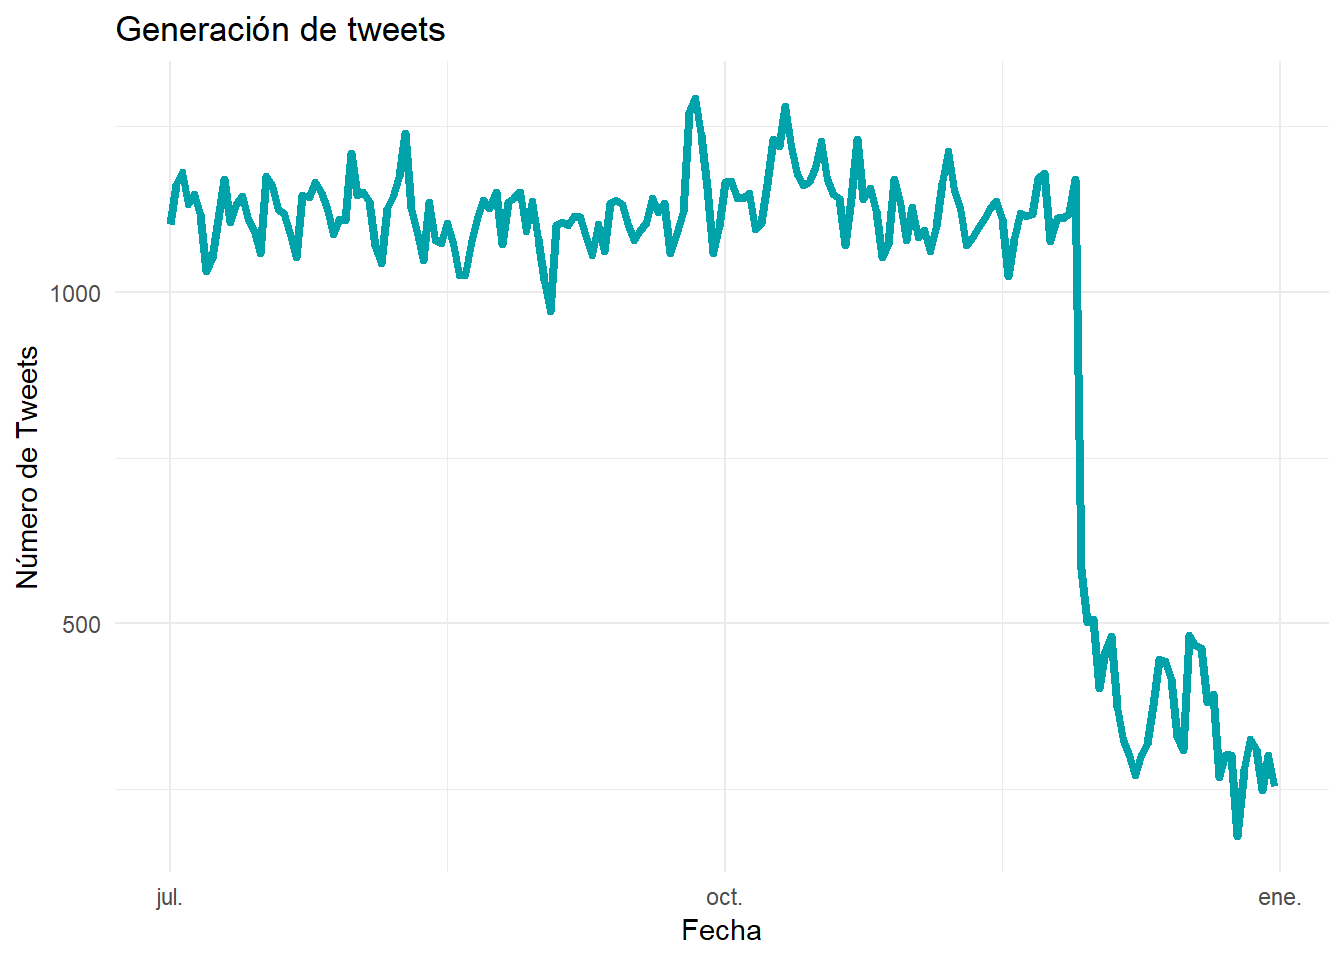
\includegraphics[scale=0.45,keepaspectratio]{imagenes/tweets_dia.png} %[width=4cm,,keepaspectratio]
	\captionof{figure}{Tweets recopilados diariamente}	
\end{center}


\begin{center}
	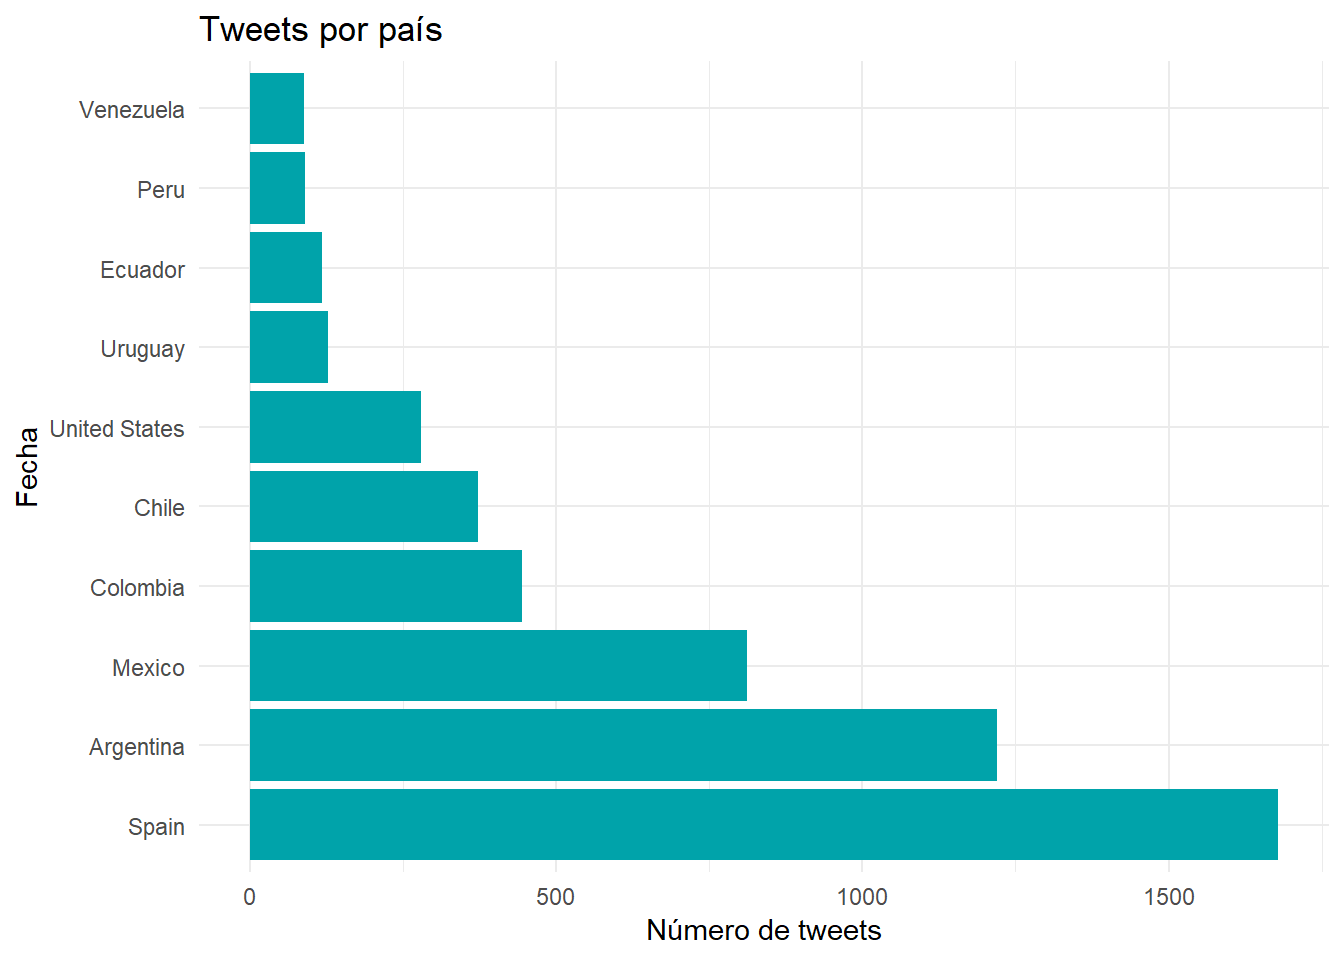
\includegraphics[scale=0.5,keepaspectratio]{imagenes/tweets_pais.png} %[width=4cm,,keepaspectratio]
	\captionof{figure}{N�mero de tweets por pa�s}	
\end{center}

Otra caracter�stica interesante es el uso de \textit{hastags} en los tweets, en total, se han recopilado 15218 hastags. En la figura 4.3 se pueden observar los t�rminos m�s utilizados. El \textit{hastag} m�s utilizado coincide con uno de los t�rminos utilizados para la recopilaci�n de los datos por el \textit{crawler}. El resto parecen estar relacionados con el programa televisivo ``Gran Hermano''. En la figura 4.4 se puede observar c�mo Espa�a es el pa�s que m�s \textit{hastags} utiliza.

\begin{center}
	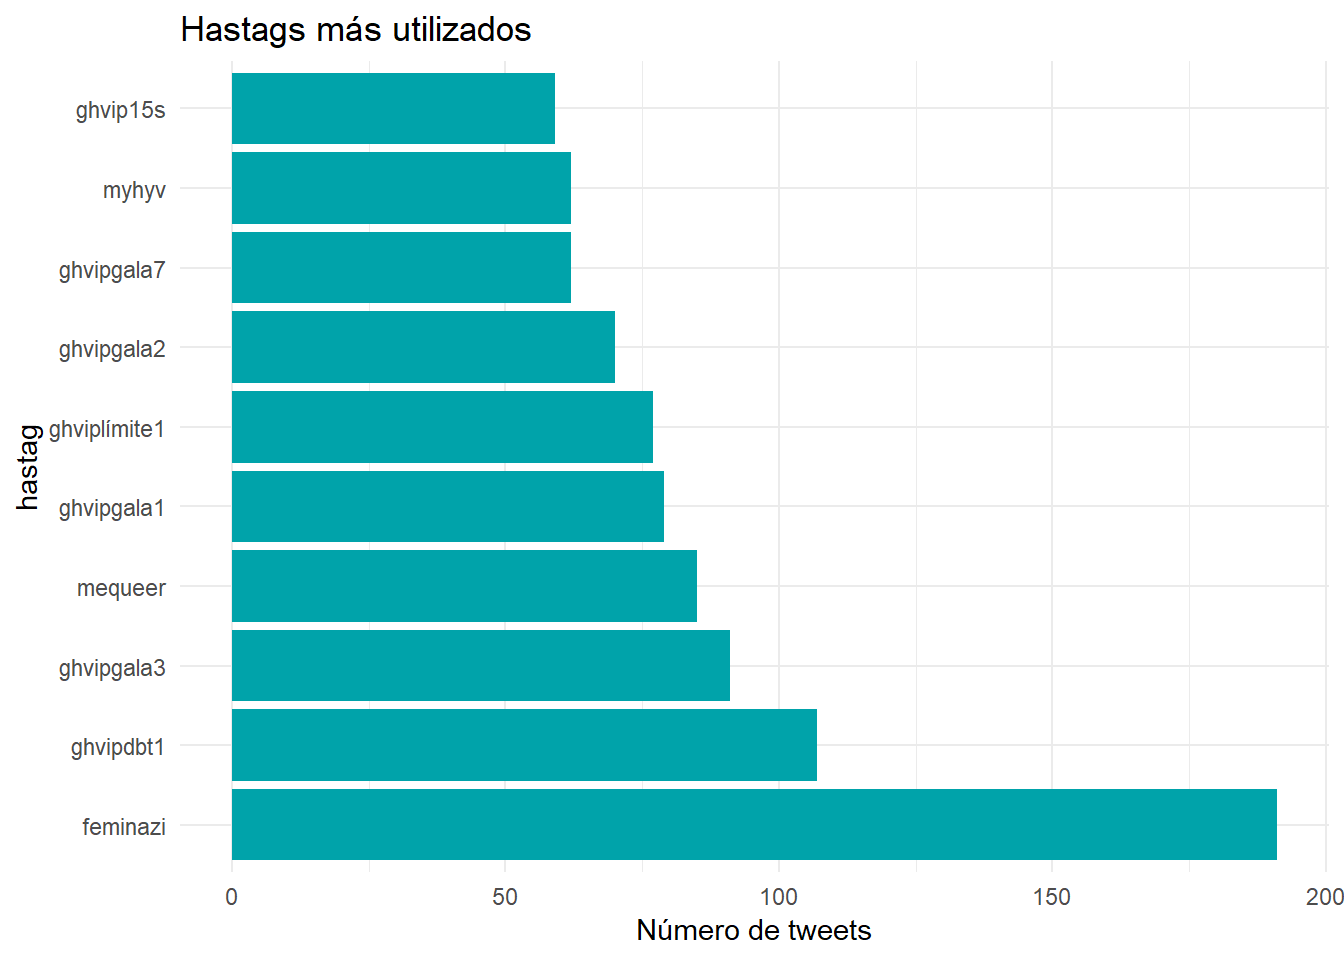
\includegraphics[scale=0.5,keepaspectratio]{imagenes/hastags.png} %[width=4cm,,keepaspectratio]
	\captionof{figure}{N�mero de hastags}	
\end{center}

\begin{center}
	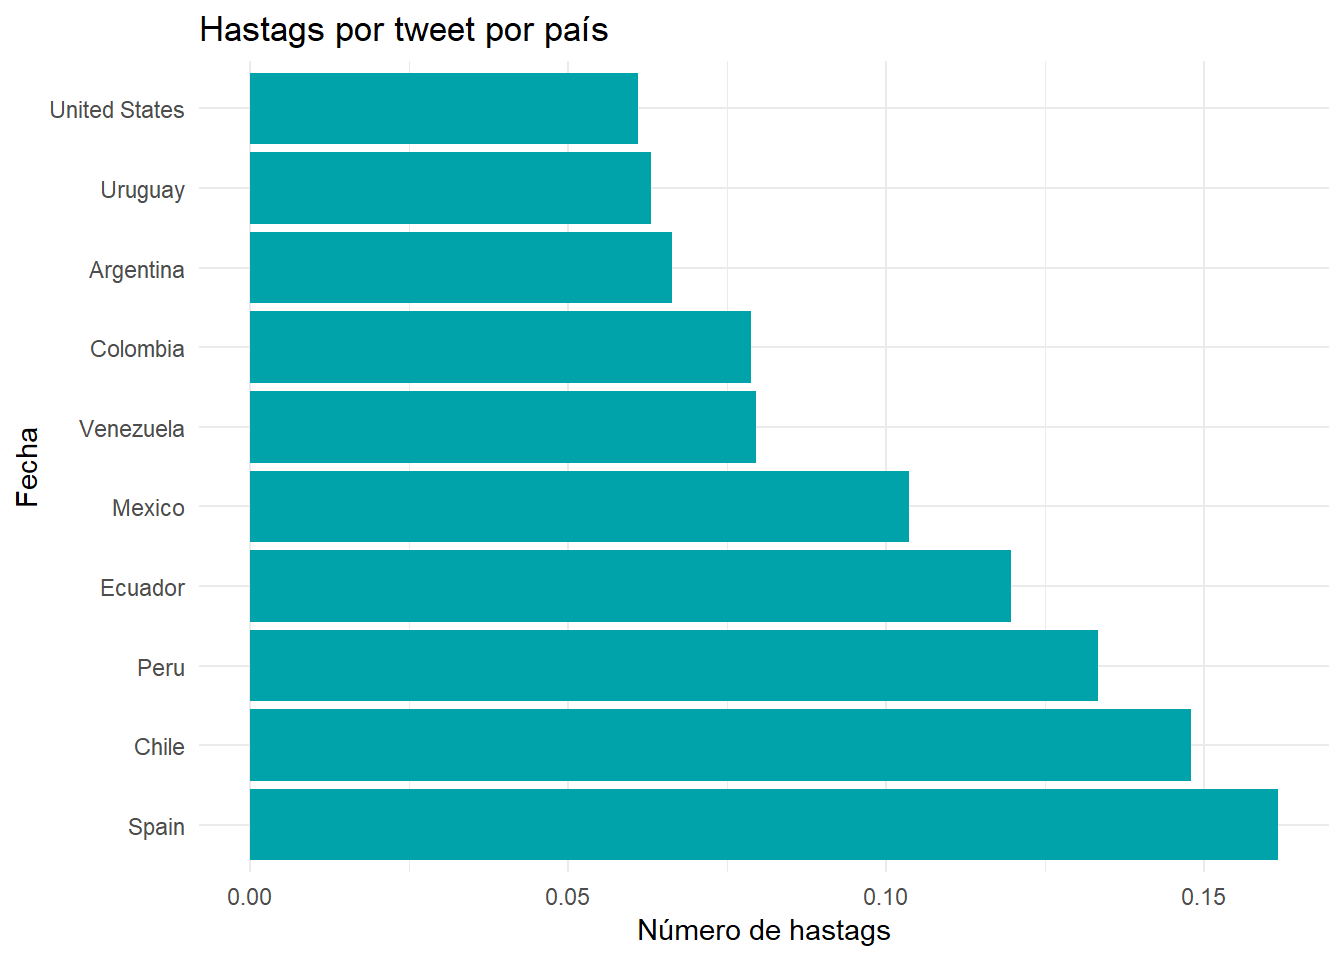
\includegraphics[scale=0.5,keepaspectratio]{imagenes/hastags_tweet_pais.png} %[width=4cm,,keepaspectratio]
	\captionof{figure}{N�mero de hastags por pa�s}	
\end{center}


Para identificar si los tweets utilizan una gram�tica adecuada, se han observado las palabras OOV (\textit{out of vocabulary}) utilizando un diccionario espa�ol. En la figura 4.5 se muestra c�mo los Estados Unidos es el pa�s con m�s OOV por tweet, llegando a 4 palabras OOV por tweet, lo que indica que los mensajes producidos contienen un gran n�mero de palabras que no se encuentran en ning�n diccionario. Esto obligar� a realizar un procesamiento para intentar normalizar este tipo de t�rminos y permitir el correcto funcionamiento del sistema de clasificaci�n.

\begin{center}
	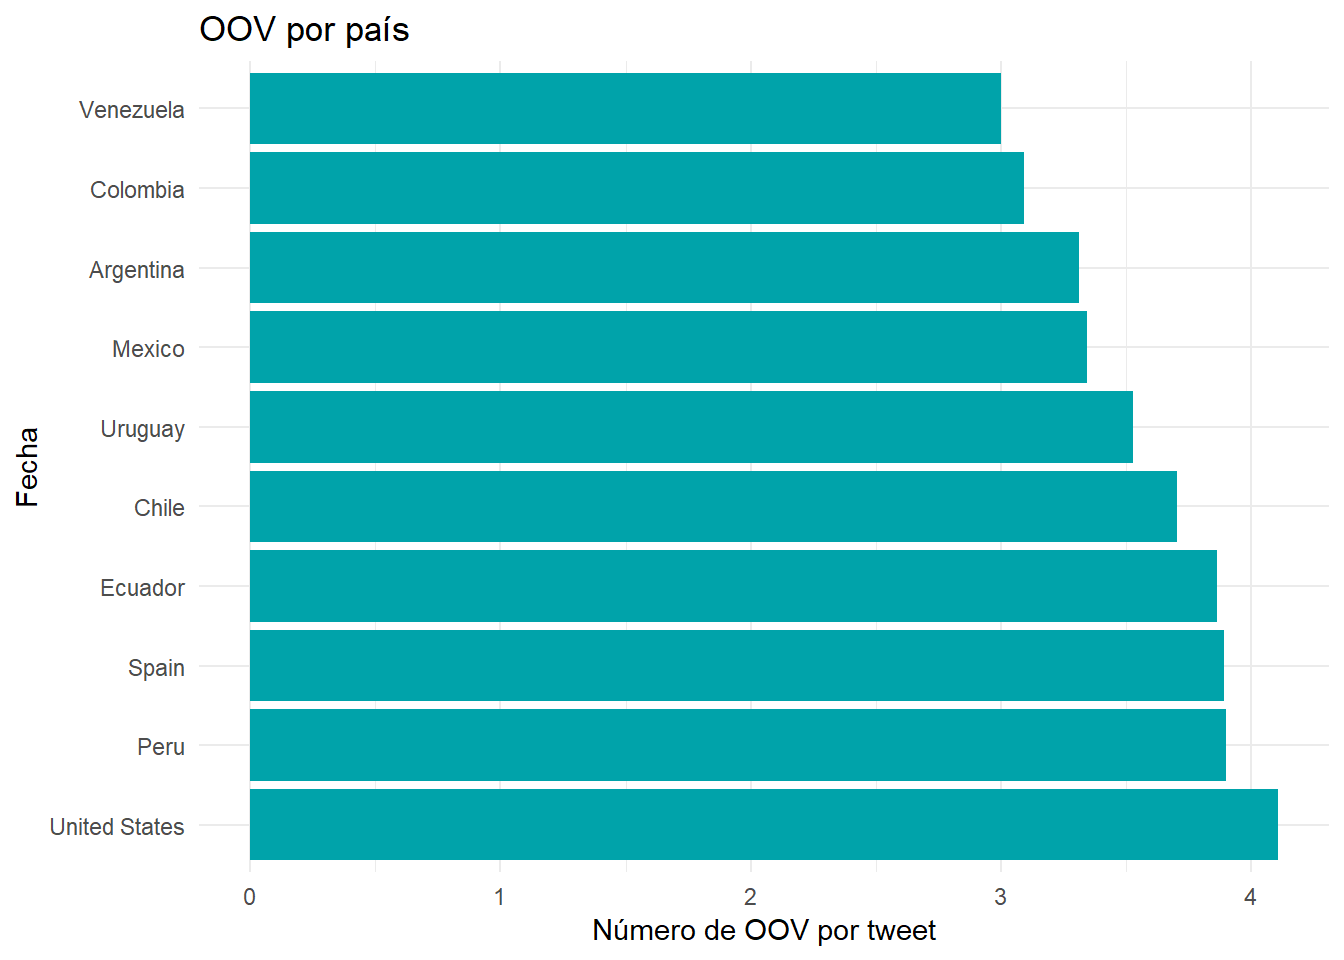
\includegraphics[scale=0.5,keepaspectratio]{imagenes/oov.png} %[width=4cm,,keepaspectratio]
	\captionof{figure}{OOV por pa�s}	
\end{center}

Por �ltimo, se han estudiado los enlaces por tweets. En total, se han recopilado 25539 enlaces para todos los mensajes. En la figura 4.6 se observa c�mo Espa�a es el pa�s que m�s enlaces por tweet utiliza.

\begin{center}
	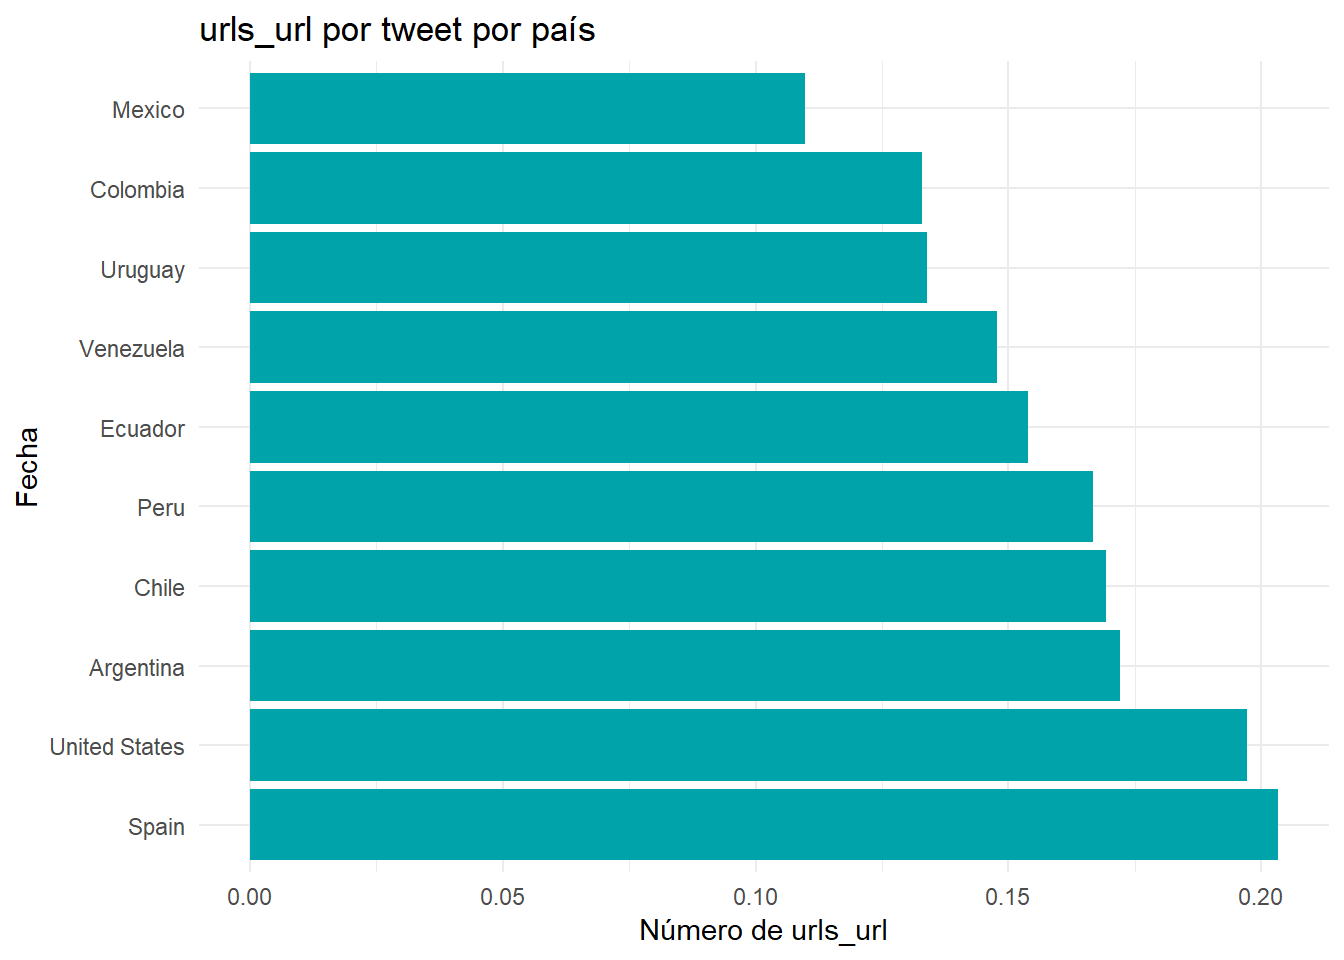
\includegraphics[scale=0.5,keepaspectratio]{imagenes/enlaces_tweet_pais.png} %[width=4cm,,keepaspectratio]
	\captionof{figure}{N�mero medio de URLs utilizadas por pa�s}	
\end{center}

\section{Etiquetado del corpus}
\label{sec:Col_Eval}

\noindent Tras la ejecuci�n del \textit{crawler}, es necesario componer el corpus a etiquetar para poder entrenar un algoritmo de aprendizaje supervisado.

Para realizar el corpus, se han utilizado las 24 expresiones con m�s de 150 tweets que se pueden observar en la tabla 4.2. Para cada expresi�n o t�rmino, se realiza un muestreo aleatorio de 150 tweets haciendo un total de 3600 tweets para ser etiquetados. Para todos los t�rminos, se ha comprobado que la separaci�n temporal entre sus tweets es m�s de un d�a, de este modo, se evitan mensajes que puedan ser conversaciones dentro del mismo d�a.

Teniendo en cuenta el objetivo principal del presente trabajo, se ha propuesto la clasificaci�n del contenido del corpus generado en tres categor�as distintas: machista, no machista y dudoso. A continuaci�n, se definen las etiquetas propuestas:

\begin{itemize}
	\itemsep0em 
	\item MACHISTA: tweets con connotaciones machistas/ofensivas hacia las mujeres. Los tweets que pertenecen a esta categor�a deben de contener actitudes discriminatorias hacia las mujeres por su sexo. Ejemplo:
	``\textit{@EmanuelGPA Lo ir�nico es que lo dice una mujer, que ``naturalmente'' deber�a callarse y dedicarse a la cocina, limpiar y criar hijos}''
	En este ejemplo, se infravalora a la mujer de un modo expreso.
	             
	\item NO\_MACHISTA: tweets que no tienen connotaciones machistas. Ejemplo:
	``\textit{�Por qu� cuando ven a una chica con pelo corto piensan que es bi, torta o marimacho? ...Capaz es solo un look o que el pelo largo le da mucho calor... Y si es...�Cual es el problema?}''
	Dentro de esta categor�a se clasifican tambi�n mensajes xen�fobos y ofensivos en general pero que no discriminan a las mujeres por su sexo. Ejemplo: 
	``\textit{@kenia773 @LuisCarlos POR CIERTO, EN TU FOTO DE PERFIL SE PUEDE OBSERVAR QUE ERES BASTANTE VARONIL, AS� QUE SI NO ERES MARIMACHO, EMPIEZA A SERLO}''
	\item DUDOSO: tweets que, dependiendo del contexto, no presente en el tweet, podr�an ser machistas (si el fragmento ofensivo se refiriese a mujeres). Ejemplo:        
	``\textit{@hazteoir @PSOE M�s vale que se marche a fregar!}''. Para poder considerar el tweet machista es necesario una referencia expresa a las mujeres, pese a que en el texto se pueda realizar una comparaci�n con una mujer mediante una expresi�n machista.                  
	
\end{itemize}

El proceso de etiquetado ha sido llevado a cabo por tres anotadores que han analizado los 3600 tweets que conforman el corpus para asignar una de las tres etiquetas propuestas. Para ello, se ha desarrollado una gu�a de etiquetado en la que se explican las etiquetas, se proponen ejemplos de cada una de ellas y se establecen las normas de entrega (ver ap�ndice). El etiquetado se llev� a cabo entre los meses de enero y marzo de 2019 mediante la herramienta ``Google Sheets'', un entorno de trabajo colaborativo online que permite la creaci�n de hojas de c�lculo.

Durante el anotado del corpus, cada uno de los tres etiquetadores propone una clase de las tres disponibles para cada tweets. Al t�rmino del etiquetado, se decidir� por votaci�n de los tres anotadores la etiqueta final. En caso de desacuerdo total entre los tres, un cuarto etiquetador decidir� la clase final para el tweet.


\subsection{Dificultades encontradas en el etiquetado del corpus}
\label{sec:Col_Eval}

\noindent Uno de los problemas m�s importantes del procesado del lenguaje natural es la ambig�edad, este fen�meno provoca que una misma expresi�n act�e con un significado distinto dependiendo del contexto en el que se encuentre. Adem�s, la complejidad inherente al uso del lenguaje, el uso incorrecto de la gram�tica del idioma y fen�menos como la iron�a o el sarcasmo dificultan la tarea de detecci�n de actitudes machistas.

En la tarea de etiquetado, una de las dificultades m�s importantes ha sido detectar se�ales textuales que indiquen comportamientos machistas debido a los efectos descritos. Para ilustrar este efecto, se pueden considerar los siguientes ejemplos:


	``\textit{@tonifreixa La zorra guardando las gallinas. �� Que se encargue Rosell �� Bueno..., cuando salga de la c�rcel. Cinismo en grado m�ximo.}''

	``\textit{@marijopellicer @radchiaru @\_lxuli Jajajaja si no sabes cuanto odio a las mujeres tengo por favor no veas enemigos donde no los hay.}''

	``\textit{Cuando subes a tu amiga la lagartona al Uber porque ya andaba malacopeando https://t.co/DcnK5ZGuL4}''

	``\textit{Mucho feminismo pero a la primera de cambio..... https://t.co/y2McecsgcT}''



En los ejemplos anteriores, los efectos del uso de la lengua dificultan la clasificaci�n en alguna de las etiquetas propuestas. En el primer ejemplo, el t�rmino ``zorra'' no es evidente si se utiliza como referencia a un animal o como un sin�nimo de prostituta.

El segundo ejemplo, se utiliza un tono ir�nico que dificulta su clasificaci�n. El usuario utiliza la expresi�n ``cuanto odio a las mujeres'' con sarcasmo por lo que no es posible afirmar que conlleve una actitud machista. En el tercer ejemplo, se podr�a entender que el t�rmino ``lagartona'' se refiere a un animal, de hecho, el tweet enlaza una imagen de un lagarto en el interior de un coche, sin embargo, en este caso el t�rmino hace referencia a prostituta. Por �ltimo, se presenta un tweet en el que se nombra al feminismo sin posicionarse en contra o a favor, en este caso sin poder detectar una actitud machista expresa.


Otra de las dificultades encontradas durante el proceso de etiquetado ha sido la clasificaci�n de tweets en los que el usuario que escribe el mensaje cita un contenido machista, en ocasiones con el que est� en desacuerdo. Este hecho se puede observar en los siguientes ejemplos:


	``\textit{Pareces una puta con ese pantal�n. - Mi hermano de 13 cuando me vio con un pantal�n de cuero}''

	``\textit{Cada vez m�s a menudo (todos lo d�as) mi padre me dice que las mujeres no deber�an recibir premios, trabajar en puestos superiores, que son putas, y que deben quedarse en casa y servir al hombre y criar hijos.}''

	``\textit{@localgothgirI Me pasa todo el tiempo, incluso, cuando me va mal, siempre recibo insultos y comentarios como ten�a que ser mujer las mujeres no deber�an jugar este juego". A veces se me quitan las ganas de seguir jugando}''

	``\textit{@mariarodd17 T�a ella diciendo cosas tipo: es que las mujeres de hoy en d�a son muy sueltas y son unas acosadoras, est�s ahora van preparadas con to y van a los hombres dici�ndoles vamos a pasar un rato que ni te cobro y ellos los pobres si tienen pareja tienen que ir preparados para no caer}''


En los anteriores, hay contexto suficiente para comprender que se cita un contenido machista como ejemplo para apoyar su desacuerdo con ese tipo de lenguaje. Sin embargo, se ha decidido incluir tanto citas, chistes o incluso cr�ticas al machismo como mensajes machistas. El objetivo principal de este trabajo ha sido identificar todo tipo de expresi�n machista para, de ese modo, determinar la cantidad de machismo existente en las redes sociales.


\subsection{Resultados del etiquetado del corpus}
\label{sec:Col_Eval}

\subsubsection{Evaluaci�n del acuerdo}
\label{sec:Col_Eval}

\noindent Para valorar el acuerdo alcanzado por los etiquetadores en su labor se ha optado por el c�lculo del coeficiente \textit{kappa de Cohen} \cite{Cohen1960}. Esta medida permite realizar una estimaci�n de la concordancia entre los etiquetadores de modo que se eval�en los resultados derivados del etiquetado manual. Una concordancia muy pobre podr�a indicar varios problemas en el proceso. Por una parte, podr�a ser que la naturaleza del problema dificulte la tarea de clasificaci�n incluso para un humano, por lo tanto, se deber�a de replantear el problema. Por otro lado, los etiquetadores podr�an no haber entendido la tarea y que sus criterios para realizarla no fueran homog�neos. El coeficiente se calcula del siguiente modo:

\[k=\frac{p_0 - p_c}{1-p_c}\]

donde $p_0$ representa el acuerdo observado relativo entre los etiquetadores o proporci�n de acierto, y $p_c$ es la probabilidad hipot�tica de acuerdo por azar. Considerando $p$ clases distintas y N el n�mero de elementos de la matriz de confusi�n:
% http://www.pacea.u-bordeaux1.fr/IMG/pdf/Kappa_Cohen.pdf

\[p_0=\frac{1}{n}\sum_{i=1}^{p}n_{ii}\]

\[p_c=\frac{1}{n^2}\sum_{i=1}^{p}n_{i\cdot}n_{\cdot i}\]

Un valor de $k = 0$ indica que la proporci�n de acuerdo es igual a la probabilidad de acuerdo por azar. Para evaluar el nivel de acuerdo seg�n el valor de esta medida se suele utilizar como convenci�n la tabla 4.3.


\begin{table}[]
	\centering
	\begin{tabular}{@{}ll@{}}
		\toprule
		\textbf{kappa} & \textbf{Tipo de acuerdo} \\ \midrule
		0.00 - 0.20 & Acuerdo muy d�bil \\
		0.21 - 0.40 & Acuerdo d�bil \\
		0.41 - 0.60 & Acuerdo medio \\
		0.61 - 0.80 & Acuerdo satisfactorio \\
		0.81 - 1.00 & Acuerdo excelente \\ \bottomrule
	\end{tabular}
	\caption{Umbrales de kappa}
	\label{my-label}
\end{table}


\subsubsection{Acuerdo etiquetadores}
\label{sec:Col_Eval}

\noindent Se realiz� una evaluaci�n de la medida kappa en dos puntos: al completar el 20\% del etiquetado de todo el corpus y al etiquetar el corpus completo. En la primera evaluaci�n, se obtuvieron los resultados de la tabla 4.4. En este caso, se valor� que para el n�mero de clases distintas este valor del coeficiente kappa era insuficiente y se revisaron los patrones de etiquetas propuestos por cada uno de los etiquetadores. De este modo, se detectaron los siguientes problemas:


% Please add the following required packages to your document preamble:
% \usepackage{booktabs}
\begin{table}[]
	\centering
	\begin{tabular}{@{}ll@{}}
		\toprule
		\textbf{} & \textbf{Kappa} \\ \midrule
		Etiquetador 1-2 & 0,5 \\
		Etiquetador 1-3 & 0,44 \\
		Etiquetador 2-3 & 0,58 \\
		\textbf{Media Etiquetadores} & \textbf{0,51} \\ \bottomrule
	\end{tabular}
	\caption{Kappa obtenido con el 20\% del etiquetado}
	\label{my-label}
\end{table}


\begin{itemize}
	\itemsep0em 
	\item El etiquetador 3 utiliz� m�s que el resto la etiqueta MACHISTA. Se concluy� que confund�a tweets por actitudes xenofobas por tweets con actitudes machistas. 
	\item El etiquetador 1 utiliz� m�s que el resto la etiqueta DUDOSO. Se revisaron sus criterios de valoraci�n de acuerdo con la gu�a de anotaci�n.    
	
\end{itemize}


Tras revisar los criterios de cada uno de los dos etiquetadores se obtuvieron los resultados de la tabla 4.4. En este caso, el coeficiente kappa alcanzado supera el valor 0.6 indicado como un resultado adecuado para este tipo de tarea.

% Please add the following required packages to your document preamble:
% \usepackage{booktabs}
\begin{table}[]
	\centering
	\begin{tabular}{@{}ll@{}}
		\toprule
		\textbf{} & \textbf{Kappa} \\ \midrule
		Etiquetador 1-2 & 0,76 \\
		Etiquetador 1-3 & 0,78 \\
		Etiquetador 2-3 & 0,74 \\
		\textbf{Media Etiquetadores} & \textbf{0,76} \\ \bottomrule
	\end{tabular}
	\caption{Kappa obtenido con el 20\% del etiquetado tras la correcci�n}
	\label{my-label}
\end{table}

Por �ltimo, se volvi� a valorar la m�trica kappa al t�rmino del etiquetado, alcanzando los resultados de la tabla 4.5. La distribuci�n de etiquetas elegida por cada anotador se observa en la figura 4.7.

% Please add the following required packages to your document preamble:
% \usepackage{booktabs}
\begin{table}[]
	\centering
	\begin{tabular}{@{}ll@{}}
		\toprule
		\textbf{} & \textbf{Kappa} \\ \midrule
		Etiquetador 1-2 & 0,68 \\
		Etiquetador 1-3 & 0,68 \\
		Etiquetador 2-3 & 0,88 \\
		\textbf{Media Etiquetadores} & \textbf{0,75} \\ \bottomrule
	\end{tabular}
	\caption{Kappa obtenido con el 100\% del etiquetado}
	\label{my-label}
\end{table}

\begin{center}
	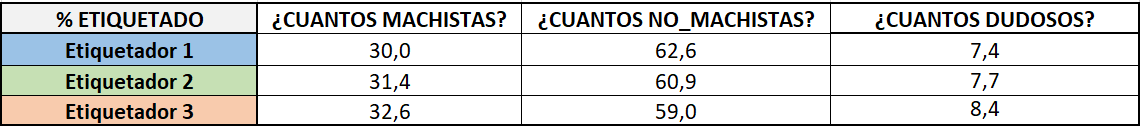
\includegraphics[scale=0.4,keepaspectratio]{imagenes/etiquetadores_final.png} %[width=4cm,,keepaspectratio]
	\captionof{figure}{Porcentaje de etiquetas elegidor por etiquetador}	
\end{center}



\subsubsection{Exploraci�n de la clase}
\label{sec:Col_Eval}

\noindent En el presente apartado se presentan los resultados derivados del proceso de etiquetado. En concreto, se va a estudiar la relaci�n de la clase asignada por los etiquetadores con dos de los tipos de atributos disponibles en el corpus: atributos num�ricos y categ�ricos.

Para el corpus final, se han asignado los valores de clase reflejados en la tabla 4.7. Como se puede observar, debido a la naturaleza del problema, los valores de la clase est�n muy desbalanceados para el valor ``NO\_MACHISTA'', contando este con m�s del 60\% de los tweets del corpus.


% Please add the following required packages to your document preamble:
% \usepackage{booktabs}
\begin{table}[]
	\centering
	\begin{tabular}{@{}lll@{}}
		\toprule
		\textbf{Etiqueta} & \textbf{Veces asignada} &  \\ \midrule
		NO\_MACHISTA & 2181 (60.58\%) &  \\
		MACHISTA & 1152 (32\%) &  \\
		DUDOSO & 267 (7.42\%) &  \\ \bottomrule
	\end{tabular}
	\caption{Distribuci�n de la clase para el corpus final}
	\label{my-label}
\end{table}

Utilizando los valores de la clase etiquetada, se han representado las variables num�ricas de las que se disponen en el corpus (figura 4.8). Dos de las m�s destacadas se pueden observar en la figura 4.9, donde se representan el tama�o de los tweets en n�mero de caracteres y de \textit{retweets}. Un aspecto a destacar es que los tweets DUDOSOS son, en media, mucho m�s cortos para que el resto de valores de la clase; sin embargo, los tweets MACHISTAS y NO\_MACHISTAS siguen una distribuci�n muy similar en cuanto al n�mero de caracteres. Asimismo, cabe destacar que los tweets DUDOSOS presentan una menor cantidad de retweets que el resto de valores de etiquetas, por tanto, estos mensajes no se propagan tanto como el resto.

\begin{center}
	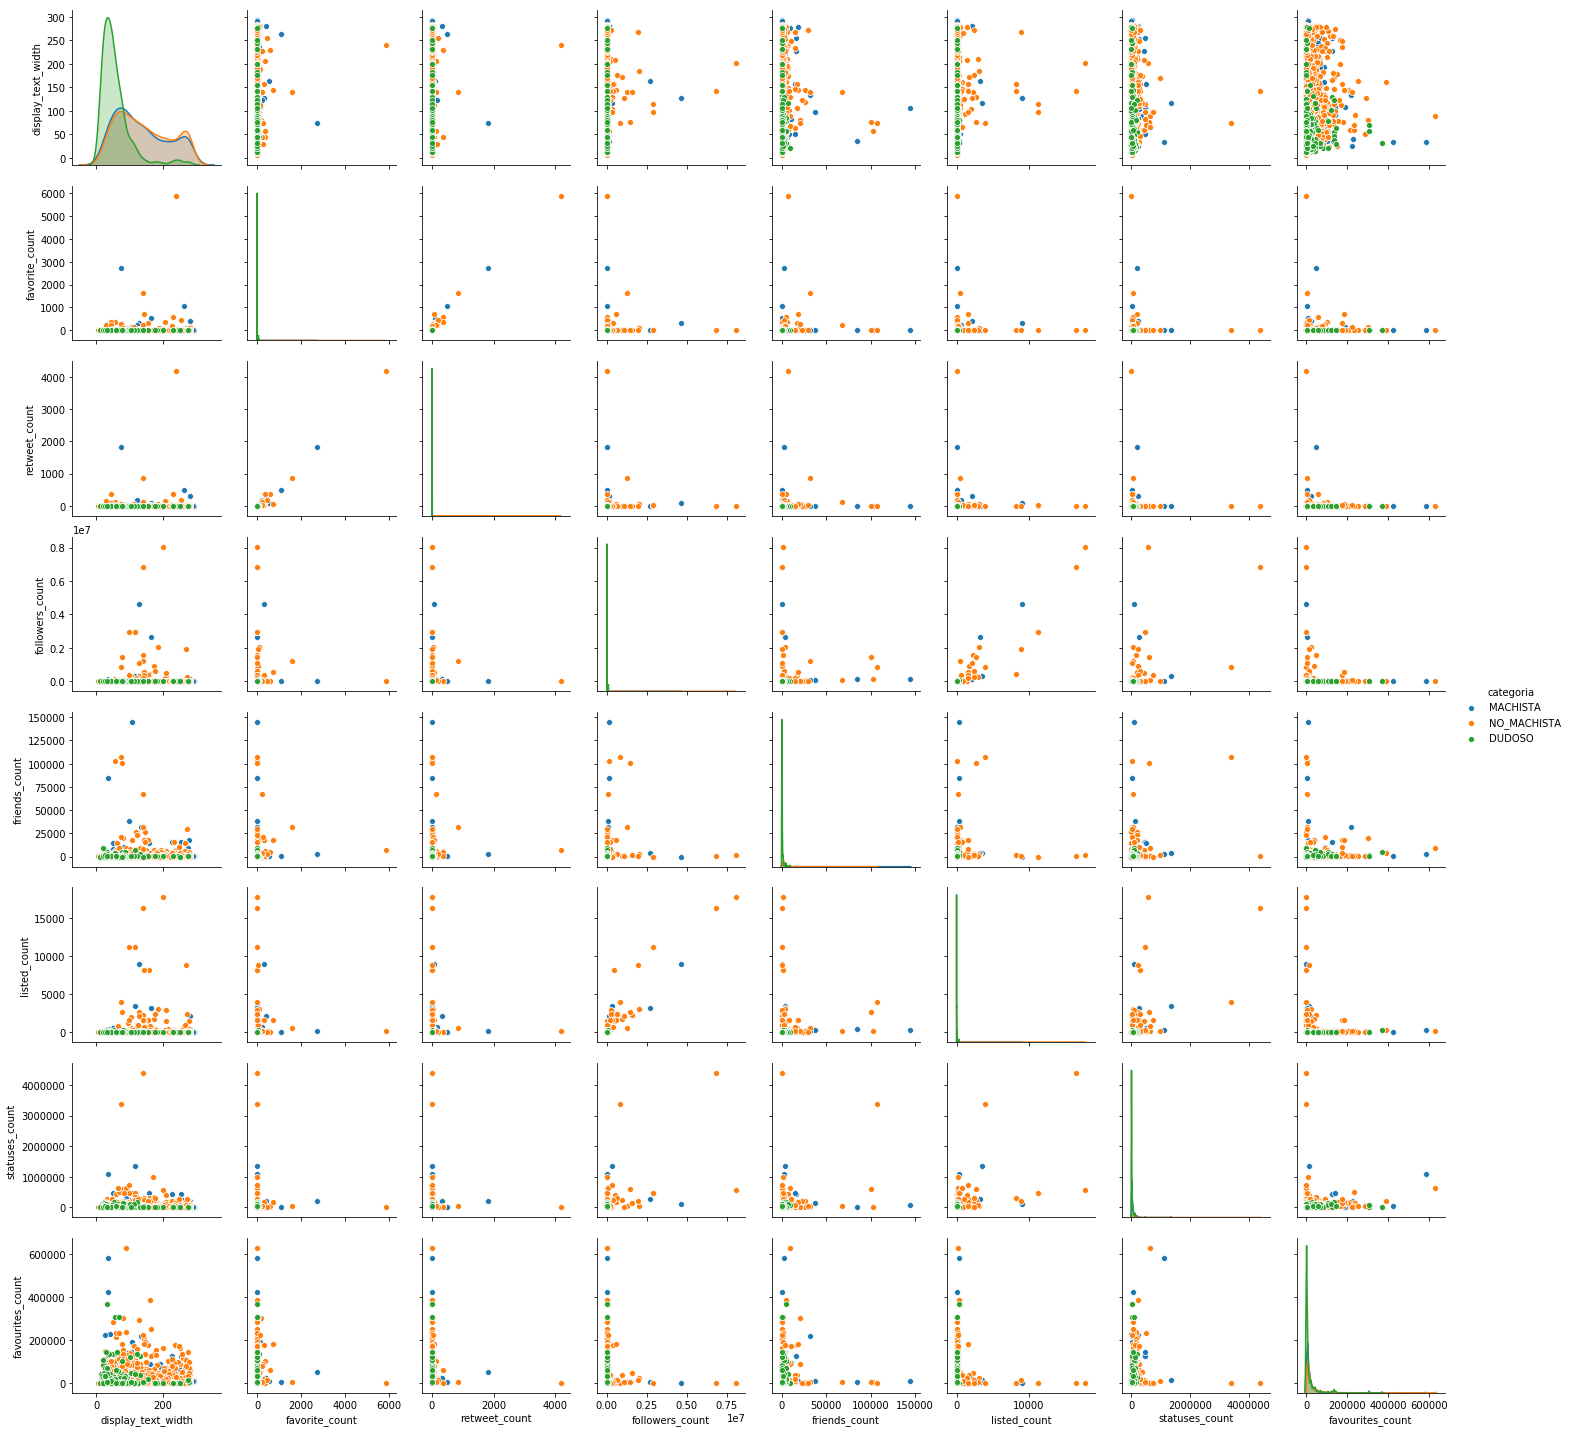
\includegraphics[scale=0.25,keepaspectratio]{imagenes/numericas_pairplot.png} %[width=4cm,,keepaspectratio]
	\captionof{figure}{Representaci�n de valores num�ricos de los tweets en funci�n de la clase}	
\end{center}


\begin{center}
	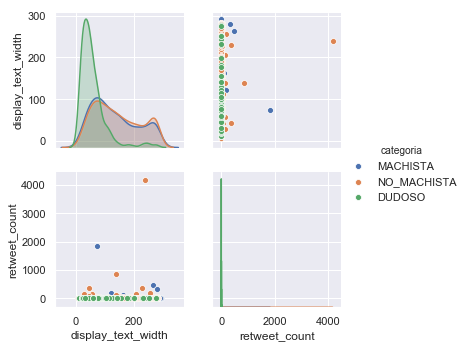
\includegraphics[scale=0.8,keepaspectratio]{imagenes/numericas_relevantes_pairplot.png} %[width=4cm,,keepaspectratio]
	\captionof{figure}{Representaci�n de valores num�ricos relevantes}	
\end{center}

\begin{center}
	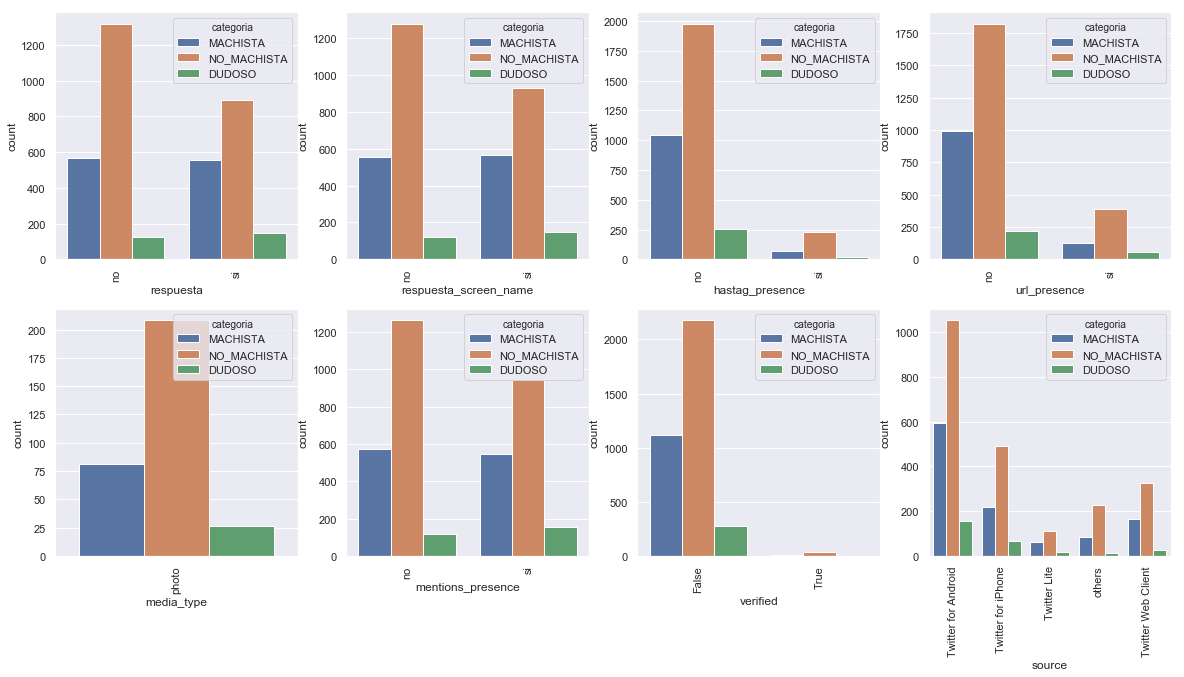
\includegraphics[scale=0.3,keepaspectratio]{imagenes/categoricas_pairplot.png} %[width=4cm,,keepaspectratio]
	\captionof{figure}{Representaci�n de variables categ�ricas}	
\end{center}

En cuanto a las variables categ�ricas, en la figura 4.10 se representan los valores para cada atributo respecto de los valores de la clase. En este caso, la distribuci�n de todas las variables categ�ricas es muy similar y no parece que la separabilidad de la clase sea tan elevada como en el caso de la figura 4.9. Un aspecto a destacar se puede observar en la variables ``respuesta'' y ``respuesta\_screen\_name'' donde parece que la probabilidad de tweet machistas es m�s elevada en el caso de que estos atributos sean afirmativos.




%%%%%%%%%%%%%%%%%%%%%%%%%%%%%%%%%%%%%%%%%%%%%%%%%%%
%%% Sistema de clasificaci�n autom�tico
%%%%%%%%%%%%%%%%%%%%%%%%%%%%%%%%%%%%%%%%%%%%%%%%%%%

\chapter{Sistema}
\fancyhead[RE]{\textsc{CAP�TULO} \thechapter. Sistema}
\label{ch:Sistema_Metodo_Caso_de_Estudio}

\noindent En el presente cap�tulo se describe el sistema autom�tico de detecci�n del machismo en redes sociales. El sistema est� basado en aprendizaje supervisado y emplea distintos atributos unificados para, posteriormente, hacer uso de un algoritmo de aprendizaje de m�quina que clasificar� los registros de entrada en 3 categor�as. De este modo, las expresiones textuales de entrada se clasificar�n seg�n el grado de machismo que presenten.

El sistema ha sido desarrollado teniendo en cuenta la naturaleza del problema tratado. En este caso, como ya se introdujo, se trata de texto en espa�ol por lo que m�todo de clasificaci�n estar� preparado para trabajar con este idioma. No obstante, la arquitectura del sistema y las t�cnicas aplicadas pueden ser adaptadas perfectamente para otros idiomas.

El sistema propuesto se divide en 3 fases principales, tal y como se puede observar en la siguiente figura.

\begin{center}
	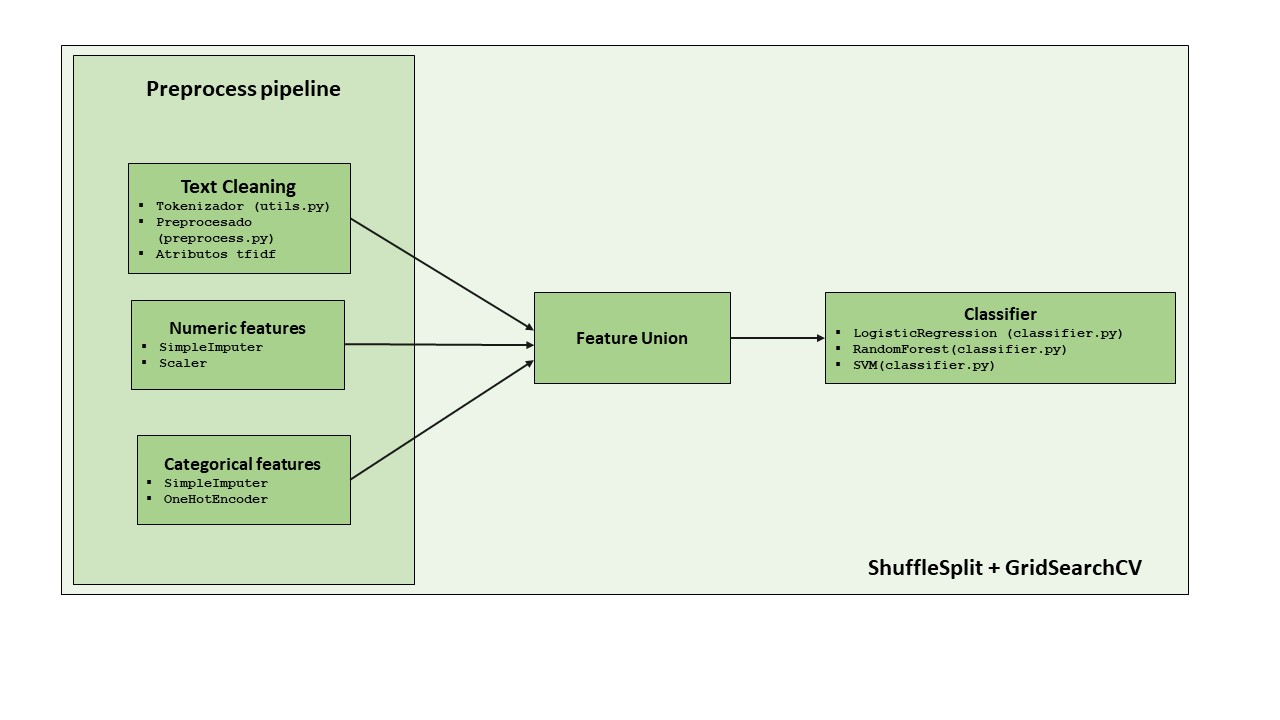
\includegraphics[scale=0.4,keepaspectratio]{imagenes/Pipeline_diagrama.jpg} %[width=4cm,,keepaspectratio]
    \captionof{figure}{Arquitectura clasificador}
	
\end{center}

En la primera etapa, se realiza un preprocesado diferenciado seg�n el tipo de atributo. En este sistema, se consideran 3 tipos de atributos distintos: variables categ�ricas, num�ricas y texto. Para cada atributo, se aplican diferentes m�todos como la tokenizaci�n, el escalado o la sustituci�n de emoticonos. Tras esto, se unifican los distintos tipos de atributos procesados en un conjunto de datos com�n que ser� la entrada de la �ltima fase. En la �ltima etapa, se emplean algoritmos de clasificaci�n supervisada con la intenci�n de obtener un modelo predictivo capaz de detectar textos machistas. Se emplean 3 m�todos distintos de aprendizaje autom�tico en este �ltimo paso: Regresi�n log�stica, Random Forest y M�quinas de vectores de soporter (SVM, ``Support Vector Machine''). Para evaluar los resultados obtenidos con estos algoritmos, se realiza una b�squeda de par�metros de entrada (GridSearchCV) y, posteriormente, se utilizan estos par�metros para realizar una validaci�n cruzada en el conjunto de testeo.


\section{Preprocesado}
\label{sec:Ejemplo_seccion}
\noindent La primera fase del sistema de clasificaci�n lleva a cabo diferentes acciones relacionadas con el preprocesado. Se realizan tareas tan importantes como la divisi�n del texto en tokens que permitir� que la informaci�n ling��stica sea tratada por las sucesivas etapas del sistema de clasificaci�n. Como se introdujo, el tipo de preprocesado depende del tipo de atributo considerado. 

\subsection{Texto}{}
\label{sec:Ejemplo_seccion}
\noindent La variable que contiene el texto contenido en el tweet es la m�s importante para la realizaci�n del sistema de detecci�n del machismo. Idealmente, se deber�a de encontrar en este atributo todas las se�ales textuales que indican si el mensaje es machista o no. Para este atributo, se aplican 3 m�todos distintos: preprocesado, tokenizador y creaci�n de atributos tf-idf.

En el preprocesado de texto se llevan a cabo las siguientes acciones:

\begin{itemize}
	\itemsep0em 
	\item Reemplazo de emojis: Se reemplazan los emojis por una descripci�n de lo que representa el dibujo. En este caso, resulta �til poder identificar el emoji que se est� utilizando ya que puede modificar el significado de la frase. Por ejemplo, en la frase de la siguiente imagen (\todo{Incluir emojis en latex}) se puede observar como el emoji permite identificar como machista la expresi�n:
\begin{center}
	
\includegraphics[scale=0.4,keepaspectratio]{imagenes/emoji_machista.png} %[width=4cm,,keepaspectratio]
	\captionof{figure}{Uso de emoji en contexto machista}	
\end{center}	
	\item Filtrado de URLs:Se reemplazan las URLs por la palabra ``\textit{twurl}".
	\item Reemplazo de acentos: Se eliminan los acentos propios del castellano.
	\item Filtrado de usuarios: Se reemplazan las menciones de los usuarios (las palabras que comienzan por "@") por la palabra ``\textit{twuser}". De este modo, se identifica cuando se utilizan las menciones omitiendo el usuario concreto.
	\item Convertidor de hastags: Se realiza una conversi�n para los \textit{hastags} que utilizan las may�sculas como separador. Por ejemplo, la frase ``\textit{\#FelizD�a}" se convertir�a a ``\textit{Feliz D�a}".
	\item Filtrado de hastags: Se reemplazan los \textit{hastags} (las palabras que comienzan por ``\#") por la palabra ``\textit{twhastag}".
	\item Convertidor a min�sculas: Se convierten todos los caracteres a min�scula.
	\item Reemplazo de exclamaciones: Se reemplazan los signos de exclamaci�n por la palabra ``\textit{twexclamation}".
	\item Reemplazo de interrogaciones: Se reemplazan los signos de interrogaci�n por la palabra ``\textit{twinterrogation}".
	\item Reemplazo de signos de puntuaci�n: Se eliminan los signos de puntuaci�n.

\end{itemize}

Para ilustrar el funcionamiento de la etapa de preprocesado, supongamos el siguiente mensaje:
\begin{center}
	
\includegraphics[scale=0.4,keepaspectratio]{imagenes/ejemplo_preprocesado.png} %[width=4cm,,keepaspectratio]
	\captionof{figure}{Ejemplo de preprocesado}	
\end{center}

Utilizando el preprocesado se obtendr�a la siguiente oraci�n transformada: ``\textit{esta es la reina de las feministas de verdad o no twinterrogation twuser thumbs\_up twurl}". Como se puede observar, se han convertido los caracteres a min�scula, se ha reemplazado el caracter de interrogaci�n, se ha sustituido la menci�n del usuario, se reemplaza el emoji por una descripci�n y se reemplaza la URL.

A partir del texto preprocesado, se realiza la tokenizaci�n de cada mensaje. Para llevar a cabo este proceso se utiliza la clase ``TweetTokenizer'' disponible en la librer�a ``NLTK''. Se trata de un tokenizador desarrollado espec�ficamente para el texto generado en Twitter. Tras la tokenizaci�n, se obtiene para cada mensaje una lista de unidades independientes que, mayoritariamente, representar�n palabras, emoticonos y signos de puntuaci�n.

Una vez realizada la tokenizaci�n del mensaje, se llevan a cabo tres procesos: filtrado de stopwords, reemplazo de abreviaturas y stemming. Las palabras vac�as o stopwords constituyen el grupo de palabras si un significado concreto, por ejemplo, art�culos, preposiciones o conjunciones. Este tipo de elementos no aportan informaci�n adicional al contexto del mensaje y, por tanto, se eliminan antes del proceso de clasificaci�n.

La tarea llevada a cabo en este trabajo presenta una dificultad a�adida por el entorno en el que se utiliza el lenguaje. En las redes sociales, y en Twitter en concreto, se publican mensajes cortos y, frecuentemente, no siguen las reglas convencionales del idioma, de este modo, el uso de abreviaturas o emoticones est� muy extendido en este tipo de plataformas. Es por ello, que realizar diccionarios espec�ficos para cada idioma que permitan normalizar este tipo de contenido es muy importante previo a la tarea de clasificaci�n. En este trabajo se utiliza el diccionario en castellano realizado en \cite{Helena2016} que compila diccionarios de palabras ``slang'', abreviaturas, contracciones y emoticones que ayudan al preprocesamiento de textos publicados en redes sociales. Un ejemplo del tipo de expresiones que se reemplazan en este proceso se podr�a ilustrar del siguiente modo: "\textit{Esta es aki la reuna de las feministas de verdad o no?}". En el ejemplo anterior, se encuentra la palabra coloquial "aki" que normalizada al espa�ol ser�a ``aqu�''.

Por �ltimo, se aplica un m�todo de stemming para reducir las palabras a su ra�z. En este caso, se utiliza el algoritmo de Porter \cite{Porter1980} desarrollado en la d�cada de los ochenta por Martin Porter y basado en un conjunto de reglas aplicadas en cascada para obtener la ra�z de las palabras.

Para ilustrar el proceso anterior, se supone el ejemplo de la figura 4.3. Aplicando el proceso de tokenizaci�n se obtendr�a la siguiente lista de tokens: ['reina', 'feminista', 'verdad', 'twinterrog', 'twuser', 'thumbs\_up', 'twurl']. Como se puede observar, se obtiene una lista de palabras, emoticonos y signos de interrogaci�n entre los cuales no se encuentran las palabras vac�as.

A partir del texto tokenizado, es necesario representar la informaci�n contenida en el texto de un modo interpretable por las etapas posteriores del sistema de clasificaci�n. Para el presente trabajo, se realiza esta representaci�n utilizando vectores de t�rminos \textit{tf-idf} mediante los unigramas de los tokens obtenidos del proceso anterior.



\subsection{Atributos num�ricos}{}
\label{sec:Ejemplo_seccion}
\noindent Otro tipo de atributo que se utiliza en el presente sistemas son los num�ricos. En este caso particular se consideran los siguientes atributos num�ricos:

\begin{itemize}
	\itemsep0em 
	\item display\_text\_width: n�mero de caracteres del tweet. 
	\item favorite\_count: n�mero de veces que el tweet ha sido marcado como favorito.
	\item retweet\_count: n�mero de veces que el tweet ha sido retwiteado.
	\item followers\_count: n�mero de seguidores del usuario que publica el tweet.
	\item friends\_count: n�mero de personas seguidas por el usuario que publica el tweet.
	\item listed\_count: n�mero de listas en las que est� inscrito el usuario que publica el tweet.
	\item statuses\_count: n�mero de tweets publicados por el usuario que public� el tweet.
	\item favourites\_count: n�mero de tweets que el usuario que public� el tweet marc� como favorito.
\end{itemize}

El uso de este tipo de atributos permite tener en cuenta distintos aspectos del contexto en el que se genera el tweet. Por ejemplo, existe un grupo de atributos como favorite\_count o retweet\_count que mide la popularidad del tweet. Por otra parte, existen campos como followers\_count que miden la popularidad del usuario que publica el tweet. Adem�s, otros campos como display\_text\_width demuestran tener una relevancia especial para los tweets etiquetados con categoria ``DUDOSO''.

En los atributos num�ricos se realizan �nicamente 2 procesos: imputaci�n de valores nulos y escalado. En este caso, se imputan los valores nulos sustituy�ndolos por 0. Para el escalado, se realiza una estandarizaci�n para que en los valores num�ricos se consiga una media nula y una desviaci�n est�ndar de uno.


\subsection{Atributos categ�ricos}{}
\label{sec:Ejemplo_seccion}

\noindent El �ltimo tipo de atributo que se emplea son los atributos categ�ricos. Para este sistema se consideran los siguientes atributos categ�ricos:

\begin{itemize}
	\itemsep0em 
	\item source: tipo de dispositivo con el que se publica el tweet. 
	\item respuesta: indica si el tweet es una respuesta a otro.
	\item respuesta\_screen\_name: nombre del usuario al que se responde.
	\item hastag\_presence: indica la presencia de ``hastags'' en el tweet.
	\item url\_presence: indica la presencia de URLs en el tweet.
	\item media\_type: indica si el tweet contiene imagenes o videos.
	\item mentions\_presence: indica la presencia de la menci�n a alg�n usuario en el tweet.
	\item verified: indica si el usuario que publica el tweet es verificado por Twitter.
\end{itemize}

Al igual que en el caso de los atributos num�ricos, el uso de algunos de estos atributos categ�ricos intentan recoger el contexto en el que se publica el mensaje, por ejemplo, el campo ``verified'' mide la influencia del usuario y los atributos ``url\_presence'' o ``media\_type'' indica si el mensaje comparte otro contenido distinto a su texto.

En los atributos categ�ricos �nicamente se aplica una transformaci�n para convertir esta informaci�n a tipo num�rico. En este caso se emplea la codificaci�n ``one-hot'' que crea un nuevo atributo por cada valor del atributo categ�rico asignando 1 � 0 seg�n la existencia o no de ese valor para cada registro.


%%%%%%%%%%%%%%%%%%%%%%%%%%%%%%%%%%%%%%%%%%%%%%%%%%%
%%% EVALUACION
%%%%%%%%%%%%%%%%%%%%%%%%%%%%%%%%%%%%%%%%%%%%%%%%%%%

\chapter{Evaluaci�n y discusi�n}
\fancyhead[RE]{\textsc{CAP�TULO} \thechapter. Evaluaci�n}
\label{ch:Evaluacion}

\todo{Explicar proceso de evaluaci�n con digramas: ShuffleSplit + Crossvalidation}
\noindent Este cap�tulo describe la metodolog�a utilizada para evaluar el sistema/m�todo o caso de estudio propuesto, a la vez que presenta los resultados obtenidos en la evaluaci�n de las diferentes tareas y sobre colecciones de evaluaci�n de distintos dominios. Algunos ejemplos de secciones pueden ser estos:

\section{Metodolog�a de evaluaci�n}
\label{sec:Met_Eval}

\subsection{M�tricas de evaluaci�n}
\label{sec:Col_Eval}

\noindent Para la evaluaci�n de los resultados en clasificaci�n textual o de documentos se utiliza com�nmente la matriz de confusi�n. Se trata de una una herramienta que representa en cada columna el n�mero de predicciones de cada clase, mientras que cada fila representa a las instancias en la clase real. En la siguiente imagen se presenta un esquema de la matriz de confusi�n:

\begin{center}
	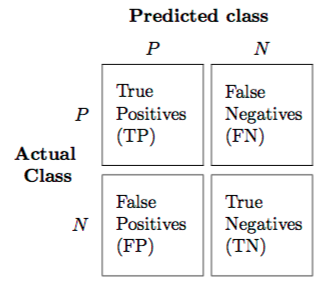
\includegraphics[width=0.5\textwidth]{imagenes/confusion_matrix_1.png} %[width=4cm,,keepaspectratio]
	\captionof{figure}{Matriz de confusi�n}	
\end{center}

Esta tabla est� formada por verdaderos positivos, verdaderos negativos, falsos positivos y falsos negativos. De este modo, si un documento es clasificado por el sistema autom�tico en la misma categor�a que la clasificaci�n manual, se considerar� como un verdadero positivo o negativo (\textit{True Positive}, TP o \textit{True Negative}, TN), mientras que si el documento es clasificado por el sistema con una categor�a diferente, se estar� ante un falso negativo o falso positivo (\textit{False Positive}, FP o \textit{False Negative}, FN).Utilizando estos cuatro componentes se calculas las medidas principales para evaluar los resultados:

\begin{itemize}
	\itemsep0em 
	\item Tasa de acierto o exactitud (\textit{accuracy}): representa el porcentaje de aciertos en relaci�n a todos los documentos clasificados.
	\[\textit{Accuracy}=\frac{TP+TN}{TP+FP+TN+FN}\]
	\item Precisi�n: representa la fracci�n de asignaciones correctas frente al total de asignaciones positivas realizadas para esa clase. Es decir, realiza una medida de la tasa de acierto para un valor de la clase.
	\[Precision=\frac{TP}{TP+FP}\]
	\item Cobertura (\textit{recall}): representa la fracci�n de asignaciones positivas respecto al conjunto real de elementos pertenecientes a la clase. Es decir, realiza una medida de la capacidad que tiene el clasificador de detectar elementos de esa clase.
	\[Cobertura=\frac{TP}{TP+FN}\]
	\item Medida-F: combina las medidas de precision y cobertura.
	\[Medida-F=\frac{2xprecisionxcobertura}{precision+cobertura}\]
\end{itemize}


\subsection{Colecci�n de evaluaci�n}
\label{sec:Col_Eval}

\subsection{L�neas base (\textit{baseline})}
\label{sec:Col_Eval}

\subsection{Experimento 1: Separaci�n 30-70 (+ optimizaci�n f1)}
\label{sec:Col_Eval}

\subsection{Experimento 2: Aplicar crossfold a todo sin tunear y con los par�metros por defecto}
\label{sec:Col_Eval}

\section{Experimento 1 (Presentaci�n de resultados y discusi�n)}
\label{sec:Metric_Eval}

\section{Experimento 2 (Presentaci�n de resultados y discusi�n)}
\label{sec:Col_Eval}

\section{Efecto del desbalanceo de la clase}
\label{sec:Resultados}




%%%%%%%%%%%%%%%%%%%%%%%%%%%%%%%%%%%%%%%%%%%%%%%%%%%
%%% CONCLUSIONES Y TRABAJO FUTURO
%%%%%%%%%%%%%%%%%%%%%%%%%%%%%%%%%%%%%%%%%%%%%%%%%%%

\chapter{Conclusiones y trabajo futuro}
\fancyhead[RE]{\textsc{CAP�TULO} \thechapter. Conclusiones y trabajo futuro}
\label{ch:Conclusiones y trabajo futuro}

\section{Conclusiones}
\label{sec:Conclu}
\noindent En este trabajo fin de m�ster se ha presentado un nuevo sistema que permite detectar el machismo en redes sociales. El sistema realiza un an�lisis supervisado y emplea distintos atributos unificados para, posteriormente, hacer uso de un algoritmo de aprendizaje m�quina que permite detectar expresiones y actitudes machistas en las redes sociales. Para cada atributo, se aplican diferentes m�todos de preprocesado como la normalizaci�n de t�rminos mediante un l�xico de \textit{slang} o la sustituci�n de emoticonos. Tras esto, se unifican los distintos tipos de atributos procesados en un conjunto de datos com�n que ser� la entrada de la �ltima fase. En esta etapa, se emplean algoritmos de clasificaci�n supervisada con la intenci�n de obtener un modelo predictivo capaz de detectar las se�ales textuales que expresan lenguaje machista.

Se ha presentado MeTwo, un corpus desarrollado en el presente trabajo y que ha sido utilizado para entrenar el sistema de clasificaci�n descrito. El corpus aportado por este trabajo cuenta 3600 mensajes etiquetados por tres anotadores para la tarea de detecci�n del machismo. Hasta la fecha, y en conocimiento del autor de este trabajo, se trata del corpus etiquetado m�s extenso disponible en castellano para la tarea de detecci�n del machismo.

Asimismo, en el cap�tulo 2, se ha realizado una extensa revisi�n del estado del arte en la detecci�n del lenguaje ofensivo, tanto sexista como de otro tipo, siendo posible detectar las principales limitaciones y problemas por resolver en la actualidad. La principal conclusi�n extra�da es que se trata de una l�nea investigaci�n muy actual y de creciente popularidad. Adem�s, se trata de una tarea compleja, en la que a�n no se ha investigado suficiente, como demuestran los escasos trabajos que tratan la detecci�n de lenguaje machista en castellano.

Uno de los principales objetivos ha sido la detecci�n de se�ales textuales que expresan lenguaje machista en castellano. En conocimiento del autor, solo una serie de publicaciones relacionadas con la competici�n \cite{AMI2018} han abordado la problem�tica desde un punto de vista pr�ctico sin una investigaci�n para la composici�n del corpus utilizado en la etapa de entrenamiento. En este trabajo, se ha experimentado con diferentes t�rminos y conceptos para componer un corpus que permita desarrollar un sistema espec�fico para la tarea y los datos recolectados. De este modo, a lo largo del trabajo, se presenta el ciclo completo para la recolecci�n de datos, preprocesamiento y construcci�n del sistema de clasificaci�n para el lenguaje natural.

Por otro lado, se ha realizado una evaluaci�n exhaustiva para determinar la viabilidad del modelo propuesto y valorar el desempe�o del sistema desarrollado. Para ello, se ha utilizado el corpus MeTwo con distintos experimentos de evaluaci�n del sistema de clasificaci�n. Asimismo, se ha estudiado el efecto del desbalanceo de la clase producida por la naturaleza del problema tratado. Los resultados obtenidos con este m�todo son prometedores y se consigue clasificar las instancias del conjunto de test con m�s de un 70\% de acierto. Pese a los resultados obtenidos, se han detectado distintas limitaciones debido a las t�cnicas utilizadas. Uno de los problemas detectados ha sido un excesivo sesgo hacia ciertos t�rminos independientemente del contexto en el que se utilicen. Por ejemplo, el t�rmino ``nenaza'' tiene gran importancia en el clasificador para la detecci�n de mensajes machistas. Asimismo, otra limitaci�n est� relacionada con los t�rminos que no se repiten a lo largo del corpus pero presentan actitudes machistas. Estos dos efectos se producen por la representaci�n textual basada en frecuencias de t�rminos y que empeora en entornos donde el uso de �stos no es homog�neo.

Otro inconveniente del sistema desarrollado es la excesiva dependencia de la presencia de t�rminos sin tener en cuenta el contexto. Debido al m�todo de representaci�n textual utilizado, el orden en el que aparecen las palabras dentro del mensaje no es importante y, por ello, el m�todo falla al detectar el machismo en textos donde no haya ning�n t�rmino que, por s� mismo, conlleve machismo en un gran porcentaje de ocasiones.

\section{Trabajo futuro}
\label{sec:Trab_Fut}

\noindent El proyecto realizado hasta el momento, presentado como trabajo fin de m�ster, ser� el punto de partida para la tesis doctoral que se pretende desarrollar en los pr�ximos a�os. Aunque los resultados obtenidos son prometedores, se han definido posibles mejoras as� como l�neas de investigaci�n futuras.

En primer lugar, el m�todo propuesto no realiza ninguna diferencia en el tipo de machismo empleado en el texto. Una posible l�nea de trabajo ser�a profundizar en los tipos de machismo existentes y realizar una ampliaci�n del etiquetado en el corpus MeTwo. En la gu�a de anotaci�n (ver Ap�ndice A) se realiza una primera exploraci�n para presentar distintos tipos de machismo, como, por ejemplo, la sexualizaci�n, el descr�dito o la dominancia.

Por otra parte, tal y como se ha podido comprobar de un modo experimental, ser�a interesante la ampliaci�n a distintos fuentes de datos como peri�dicos, webs u otras redes sociales. En algunos experimentos, como en el apartado 6.4, se ha concluido que la bondad de los resultados podr�a ser mayor si se dispusiera de una mayor cantidad de informaci�n.

Asimismo, ser�a recomendable profundizar en las t�cnicas para la clasificaci�n autom�tica, por ejemplo, t�cnicas basadas en redes neuronales que alcanzan unos resultados prometedores en tareas relacionadas con el procesamiento de texto como BERT \cite{Jacob2019}. Este tipo de t�cnicas, junto con representaciones textuales basadas en \textit{word embedding}, podr�an ayudar a paliar algunas de las limitaciones detectadas en el sistema propuesto como, por ejemplo, la consideraci�n del contexto en el que se utilizan los t�rminos machistas.

Otra l�nea de trabajo futura podr�a ser la adaptaci�n del sistema para el idioma ingl�s. Debido al dise�o de este m�todo, se podr�a adaptar f�cilmente para ser capaz de detectar expresiones machistas en otros idiomas.

Adem�s, ser�a recomendable la creaci�n de un l�xico machista espec�fico para el espa�ol que permita a�adir atributos en el entrenamiento del sistema para detectar aquellos t�rminos que m�s se repitan en los mensajes machistas. Este tipo de enfoque ha demostrado su efectividad en trabajos similares \cite{Wahyu2018} y se podr�an implementar mediante l�xicos disponibles en la bibliograf�a \cite{Mauro2016}.

Finalmente, como salida del sistema, ser�a interesante la creaci�n de un portal web que permita, mediante distintos tipos de visualizaciones, explorar los tipos de machismos en Espa�a, Europa o todo el mundo. Podr�a servir para detectar y prevenir los tipos de machismos en cada zona geogr�fica, indicar los t�rminos machistas m�s empleados y los medios m�s afines para propagar este tipo de mensajes.



%%%%%%%%%%%%%%%%%%%%%%%%%%%%%%%%%%%%%%%%%%%%%%%%%%%
%%% BIBLIOGRAF�A
%%%%%%%%%%%%%%%%%%%%%%%%%%%%%%%%%%%%%%%%%%%%%%%%%%%
\bibliographystyle{fullname_esp}
\cleardoublepage
\addcontentsline{toc}{chapter}{Bibliograf�a}
\chapter*{Bibliograf�a}
\fancyhead[RE]{BIBLIOGRAF�A}
\fancyhead[LO]{BIBLIOGRAF�A}
\bibliography{Bibliografia}


\newpage
\newpage

%%%%%%%%%%%%%%%%%%%%%%%%%%%%%%%%%%%%%%%%%%%%%%%%%%%
%%% APENDICES SI PROCEDE (COMENTAR)
%%%%%%%%%%%%%%%%%%%%%%%%%%%%%%%%%%%%%%%%%%%%%%%%%%%
%\appendix
%\chapter{Publicaciones}
%\label{ch:publicaciones}
%\fancyhead[RE]{\textsc{AP�NDICE} \thechapter. Publicaciones}
%\fancyhead[LO]{\textsc{AP�NDICE} \thechapter. Publicaciones}

%Publicaciones derivadas del trabajo realizado.

\appendix
\chapter{Gu�a de anotaci�n}
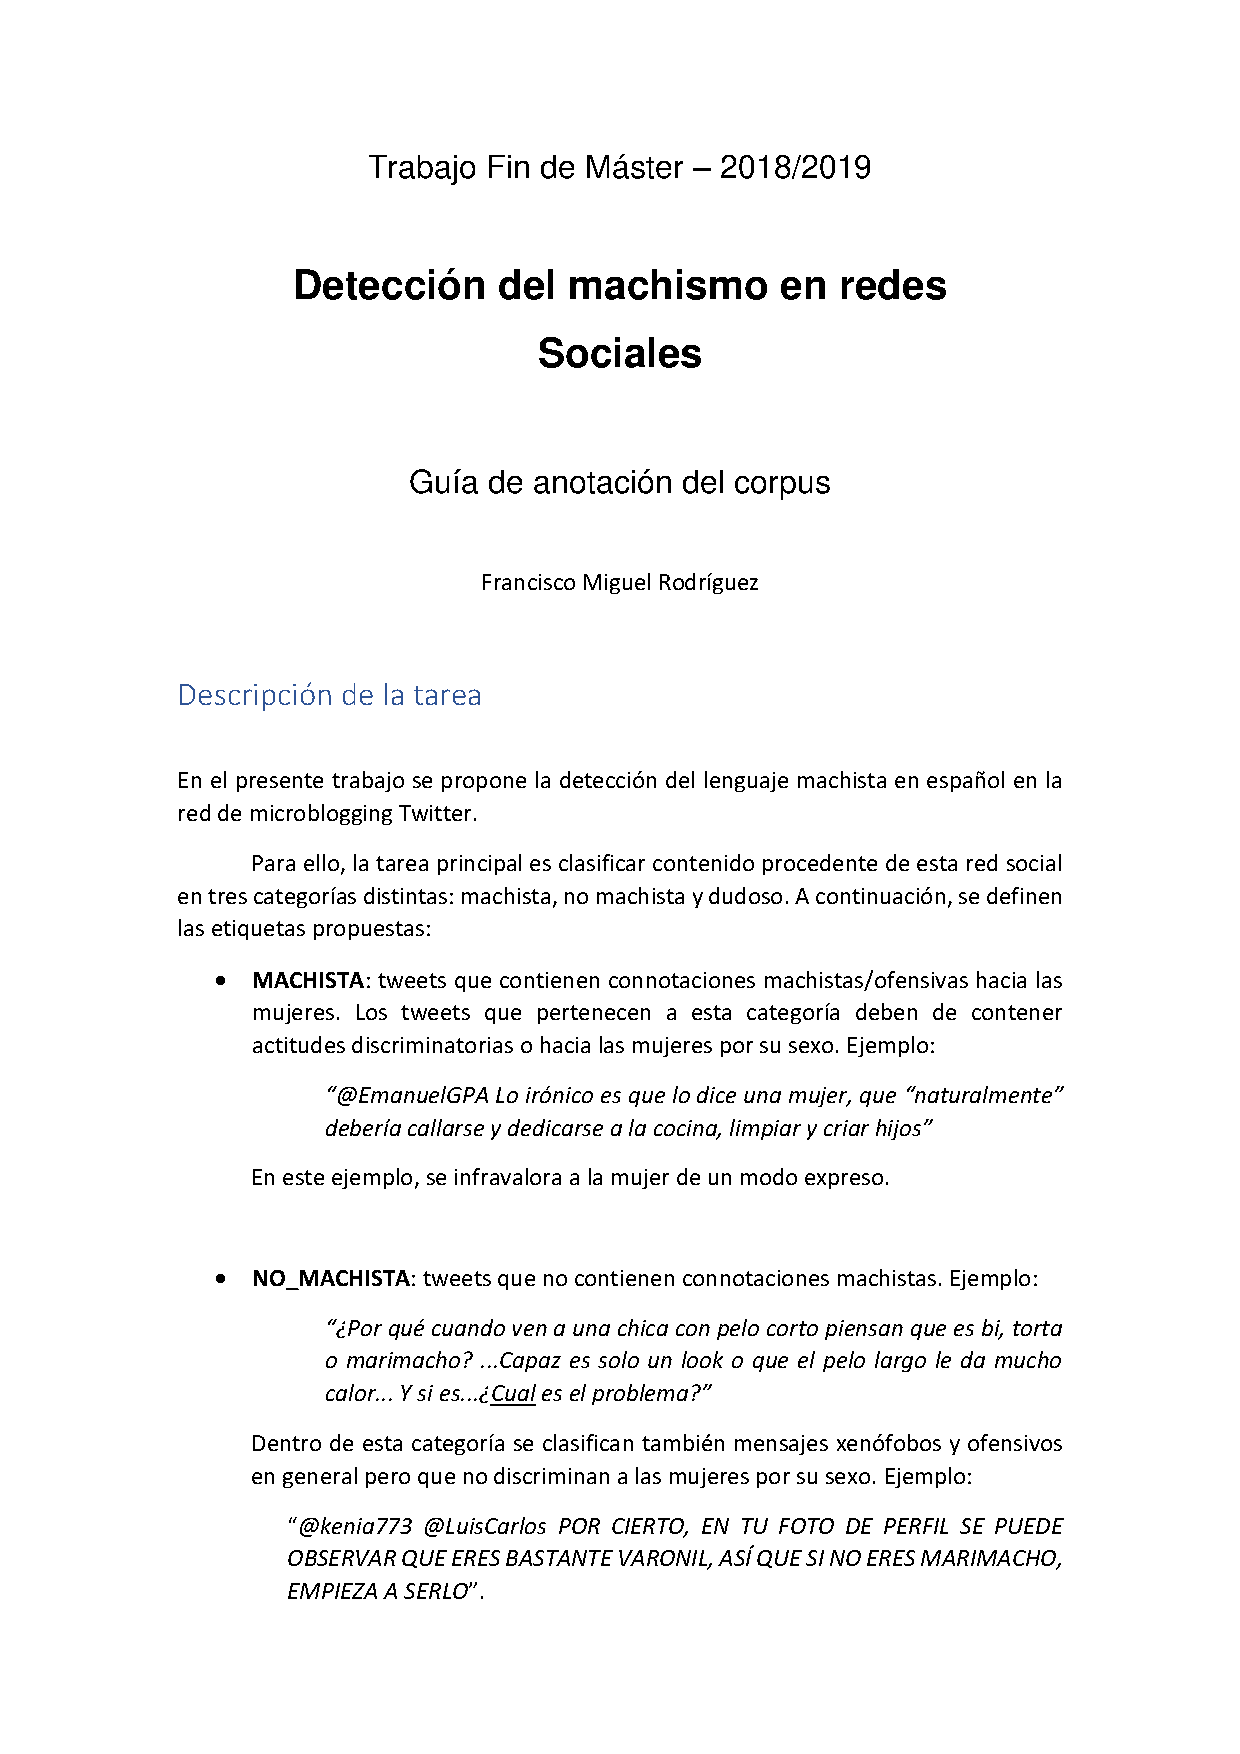
\includepdf[pages={1-7}]{Guia_anotacion.pdf}

%%%%%%%%%%%%%%%%%%%%%%%%%%%%%%%%%%%%%%%%%%%%%%%%%%%
%%% lISTA DE TAREAS PENDIENTES.
%%%%%%%%%%%%%%%%%%%%%%%%%%%%%%%%%%%%%%%%%%%%%%%%%%%
\newpage
\newpage
%Eliminar si no hay todo's
%\listoftodos


\end{document}

%%%%%%%%%%%%%%%%%%%%%%%%%%%%%%%%%%%%%%%%%%%%%%%%%%%
%%% SCRIPT FINAL DE TODO'S O TAREAS PENDIENTES.
%%%%%%%%%%%%%%%%%%%%%%%%%%%%%%%%%%%%%%%%%%%%%%%%%%%
% Make the margin par
\marginpar{%
    \begin{tikzpicture}[remember picture]%
        \draw node[notestyle] (inNote)
                 {#1};%
    \end{tikzpicture}%
}%
%
\begin{tikzpicture}[remember picture, overlay]%
    \draw[connectstyle]
        ([yshift=-0.2cm] inText)
            -| ([xshift=-0.2cm] inNote.west)
            -| (inNote.west);
\end{tikzpicture}%

}% 